\chapter{IPBPMs Movers}\label{s:annexB}
\section{System Description}
At the ATF2 IP region, inside the vacuum chamber, the BPMs positioning system has been installed during the first two weeks of July 2013. It moves two independent blocks: Block IPAB and Block IPC. Each block has three degrees of freedom: vertical, lateral and pitch angle, using using four piezo-movers per block: three vertical and one horizontal.\par
Movers made by the german company ``PI'' electronics moves IPC and the french company ``Cedrat Technologies'' moves IPAB.\par
\subsection{The Piezo Movers}
Piezo mover changes its position as a function of voltage. Each one of the eight movers has its own control electronics block composed of: 
\begin{itemize}
 \item The piezo-mover to generate the displacement.
\item The strain gauge, used by the control box for feedback.
\item The control box (module provided by the manufacturer) to:
\begin{itemize}
 \item Set piezo-mover high voltage to induce the motion of the piezo-mover.
 \begin{itemize}
\item PI module E-621
\item CEDRAT module LA75
\end{itemize}
\item Read strain gauge to know the piezo-mover position.
\begin{itemize}
\item PI module E-621 (same as control)
\item CEDRAT module SG75
\end{itemize}
\item Set feedback operation (ON/OFF).
\item Set control mode: internal or external setting point. External mode is used.
\end{itemize}
\item PLC channel to:
\begin{itemize}
\item Set voltage to the setting point input in the control box.
\item Read voltage from control box output proportional to piezo-mover position.
\end{itemize}
\end{itemize}

\subsection{Electrical connections}
Figure \ref{f:conndiag} shows the electrical connections diagram between the movers displacement system components. It shows the connexion to the local network by Ethernet, the DACs and ADCs used to set and read the voltage levels, the connection to the dedicated control boxes, a linking box to match the cable connectors, the 25~m cable to connect to the vacuum chamber flanges inside the ATF tunnel, the movers, and temperature probes.\par
\begin{figure}[hbt]
\hspace*{1.4cm}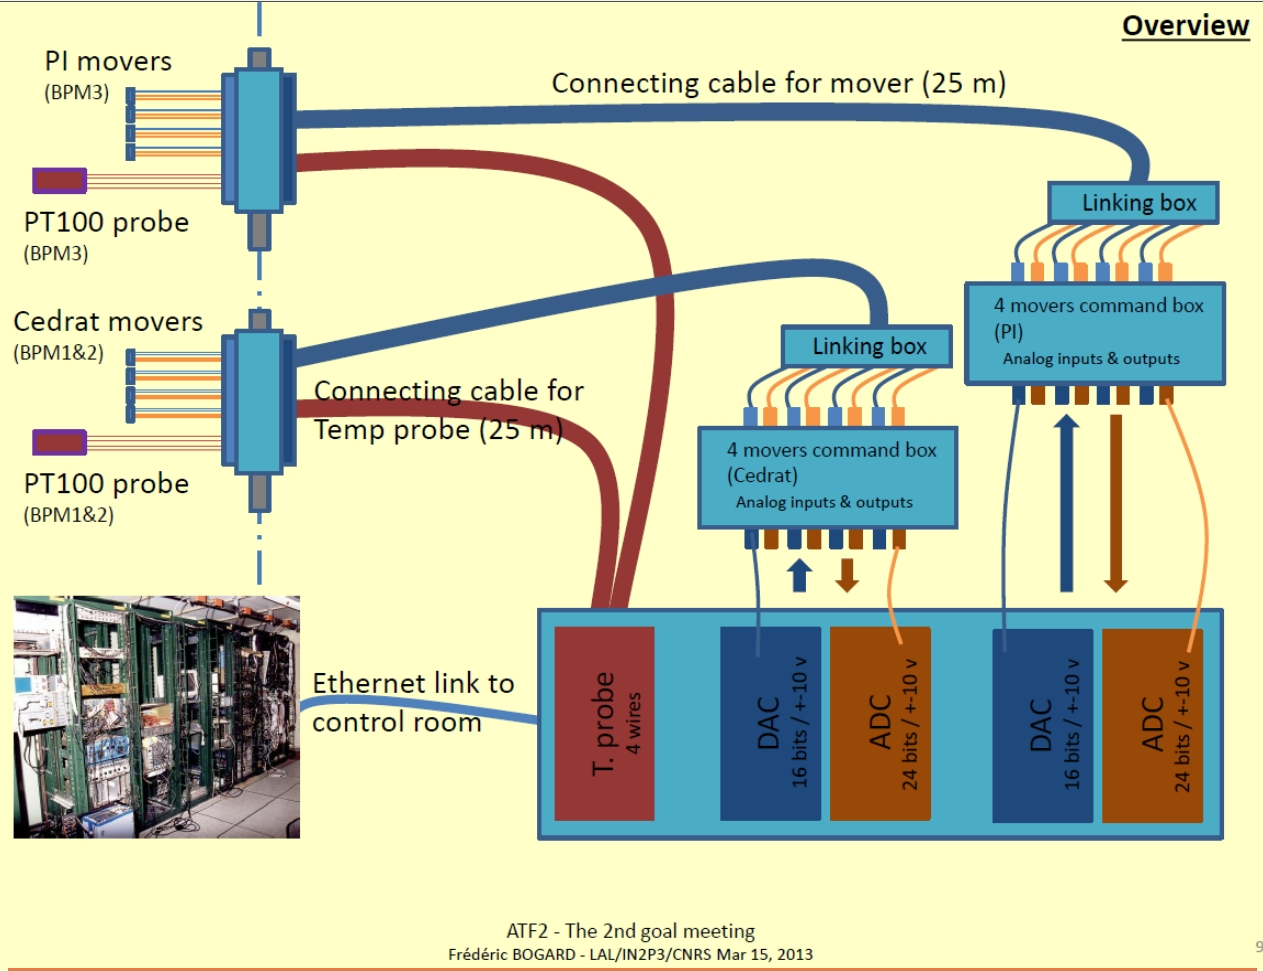
\includegraphics[angle=0,scale=0.3]{link.jpg}\caption{Piezo mover system connection diagram.}\label{f:conndiag}
\end{figure}
% \begin{figure}[htb]
%  \centering
% \begin{tikzpicture}
%   \node (img1) {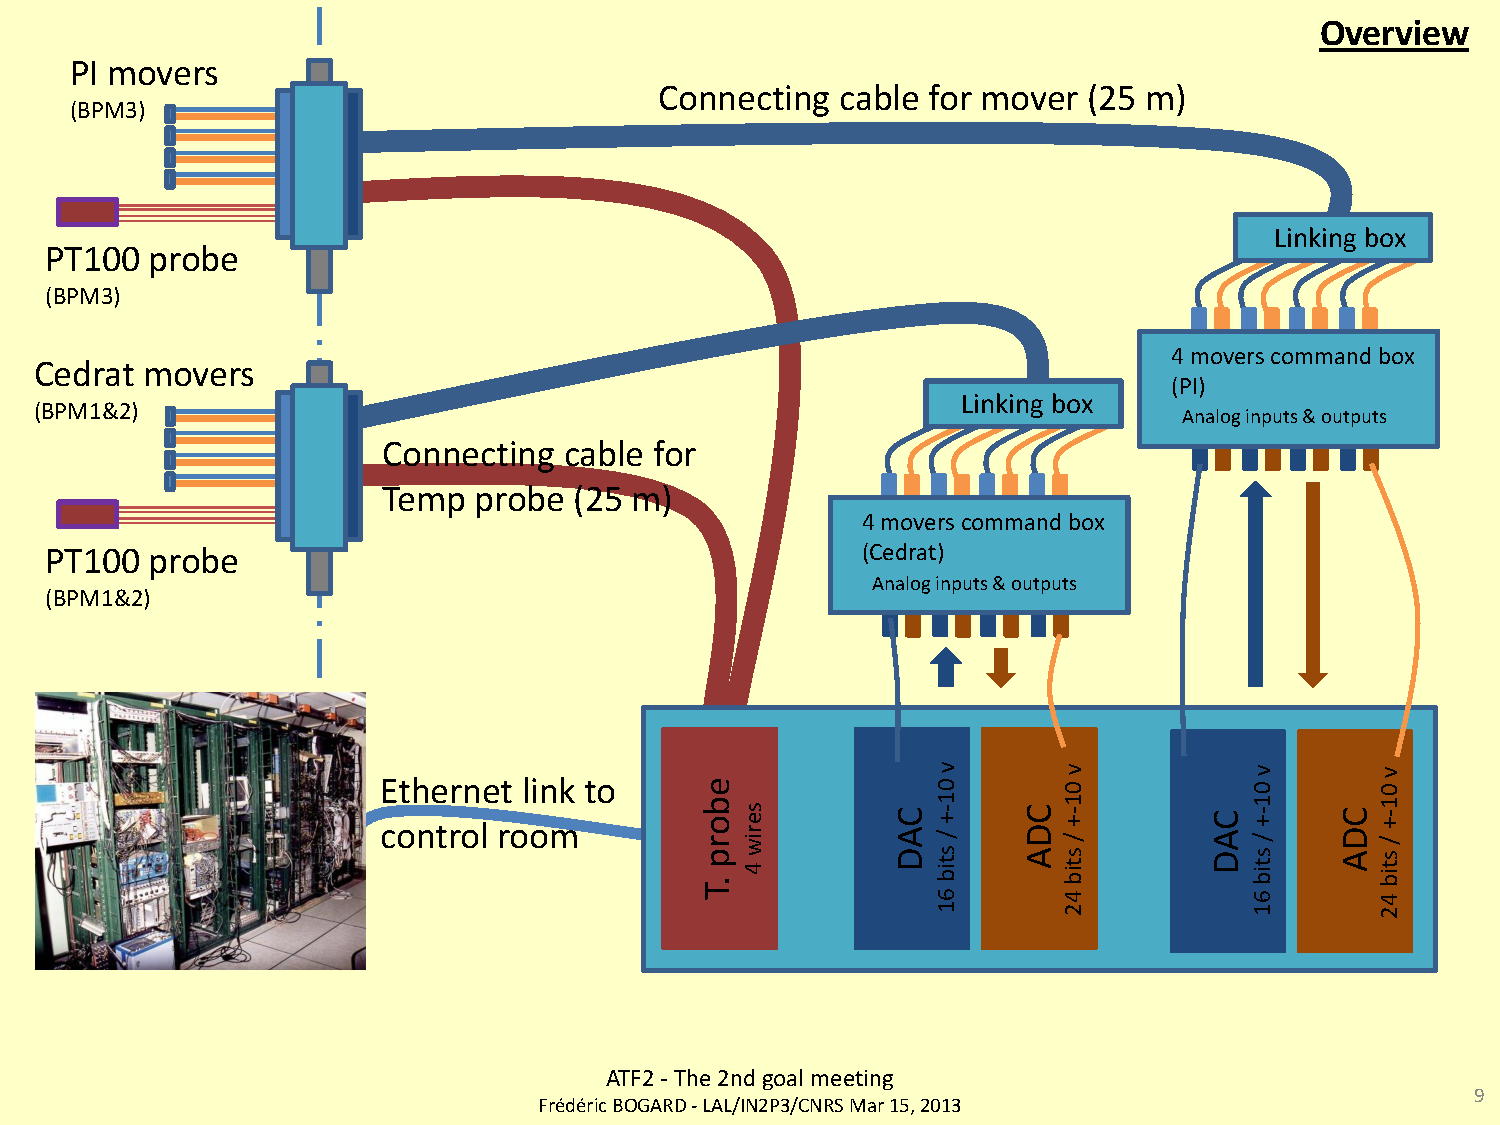
\includegraphics[scale=0.45,angle=0]{elect01.pdf}};
%  %\pause
%   \node (img2) at (-4.2,-3) {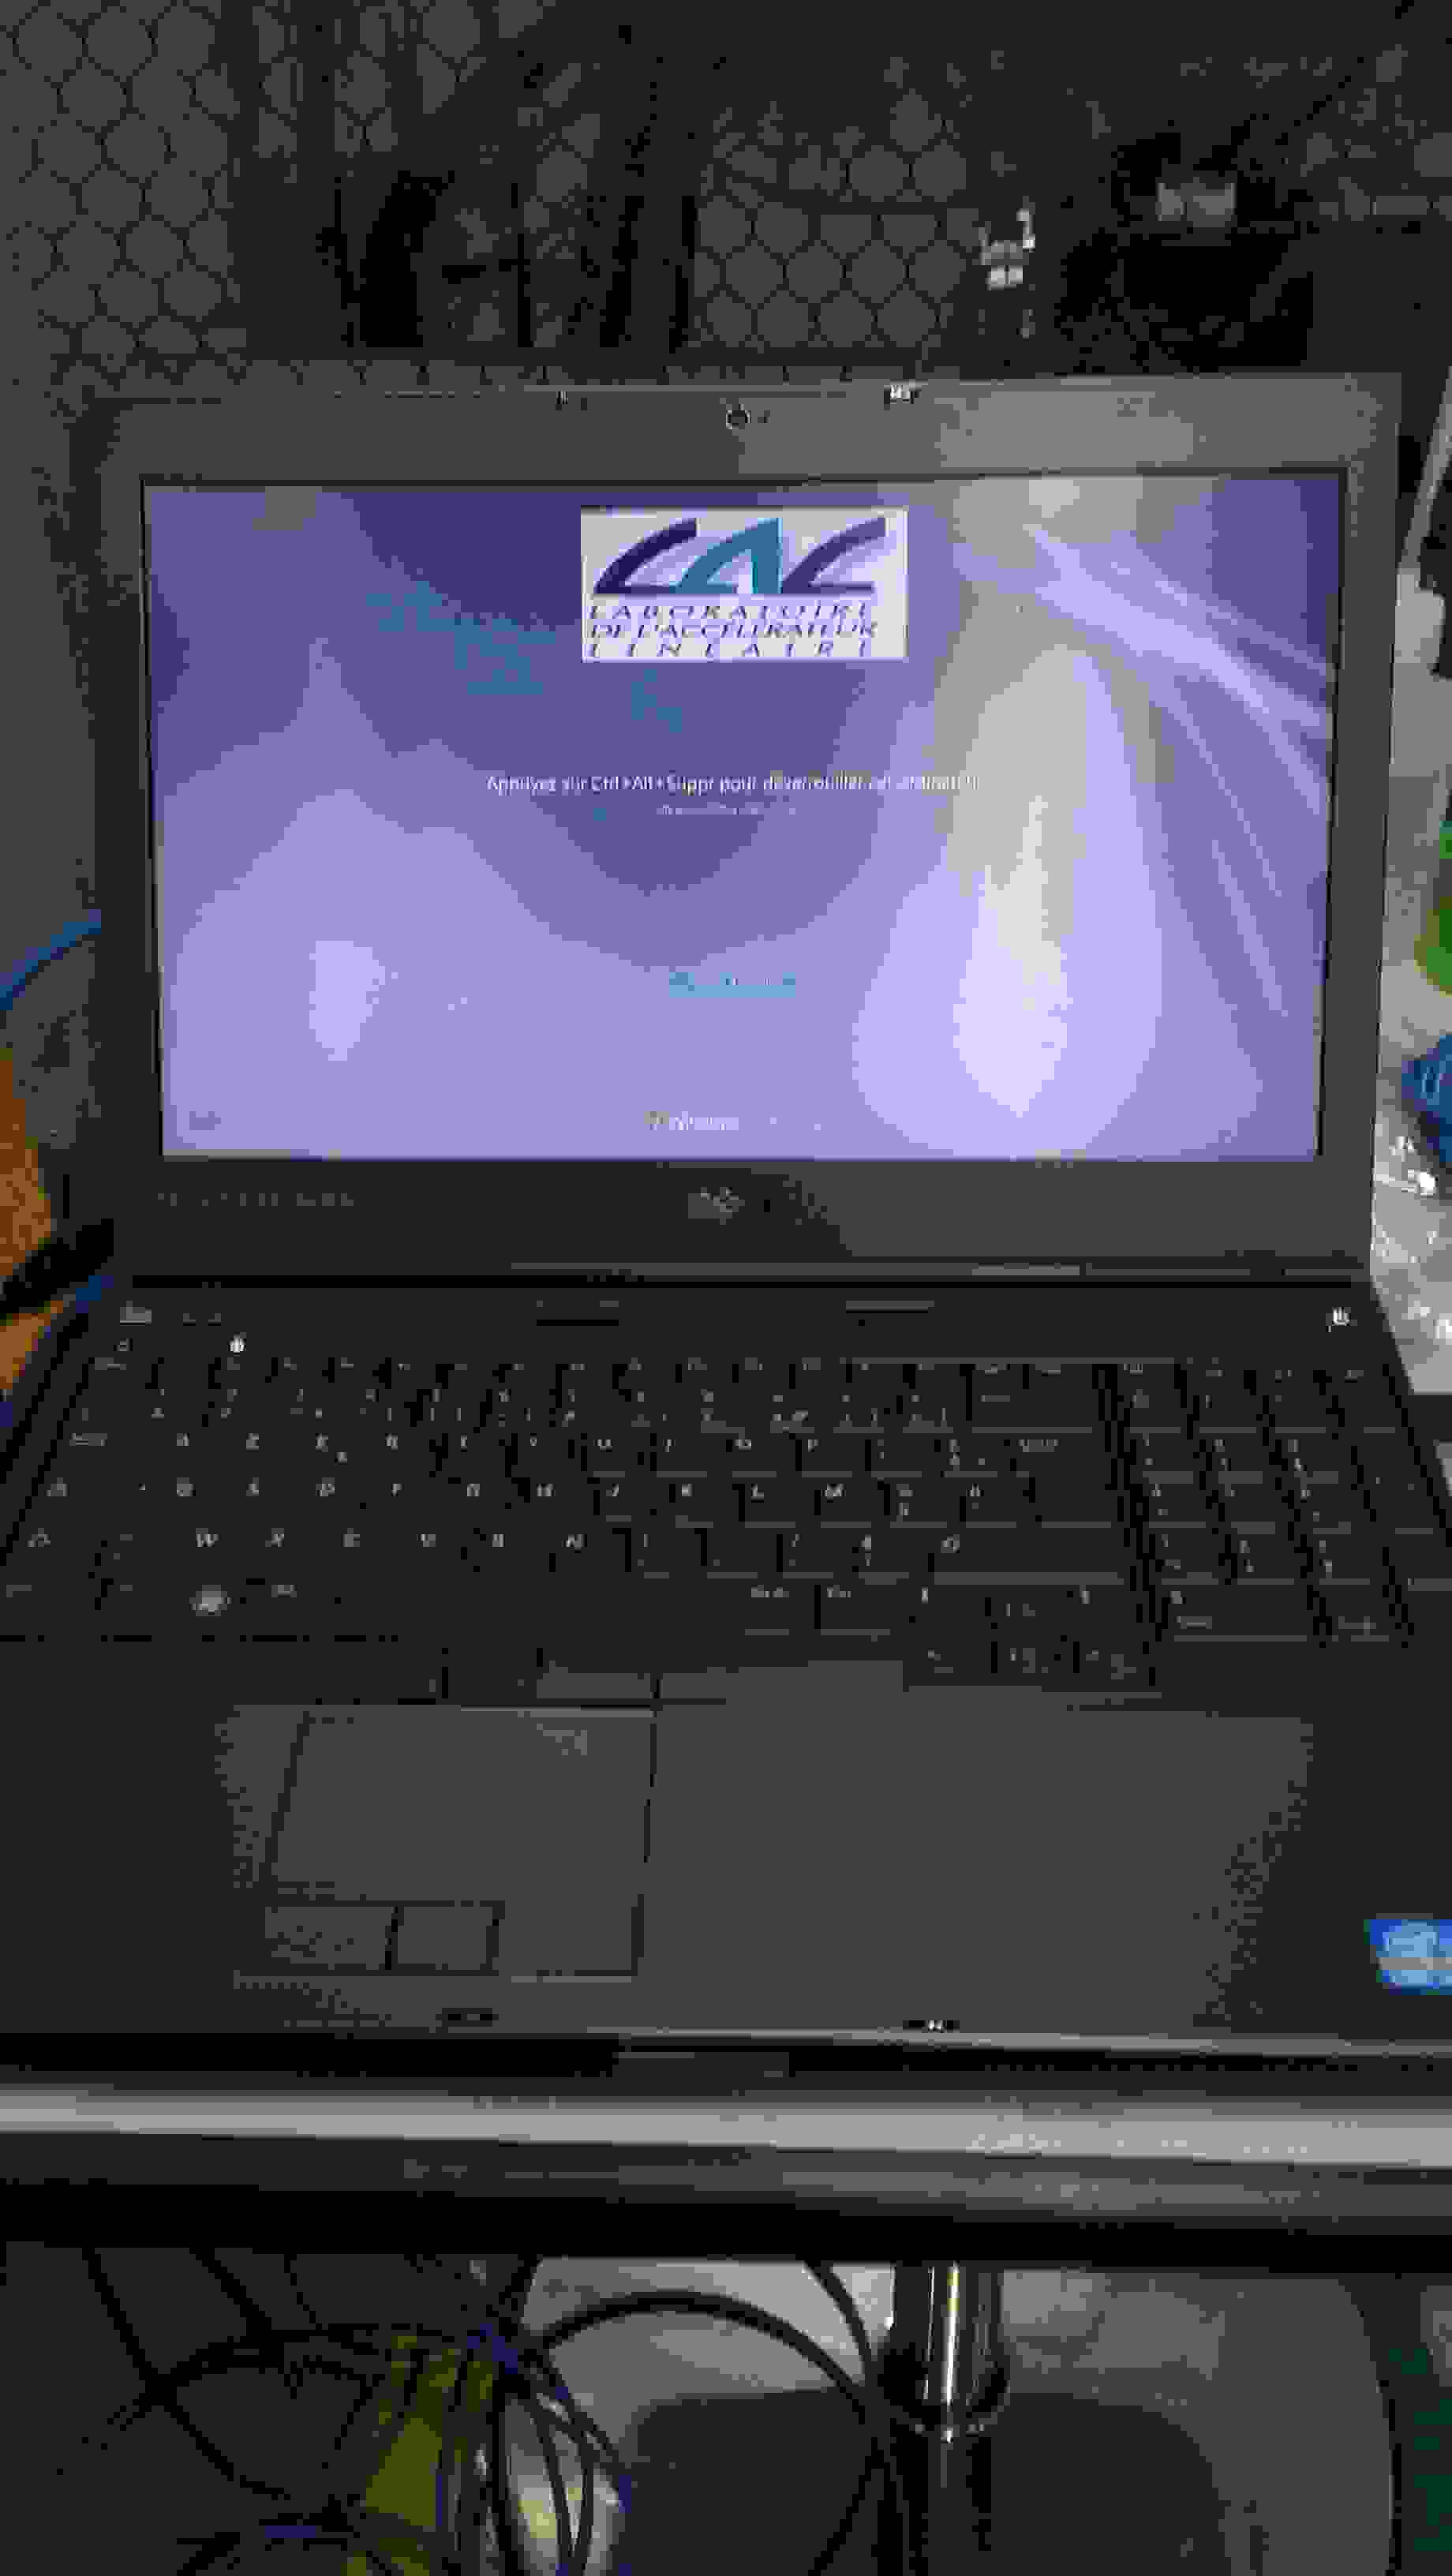
\includegraphics[scale=0.039,angle=0]{ima02a.jpg}};
% %   \pause
%   \node (img3) at (2.2,-2.1) {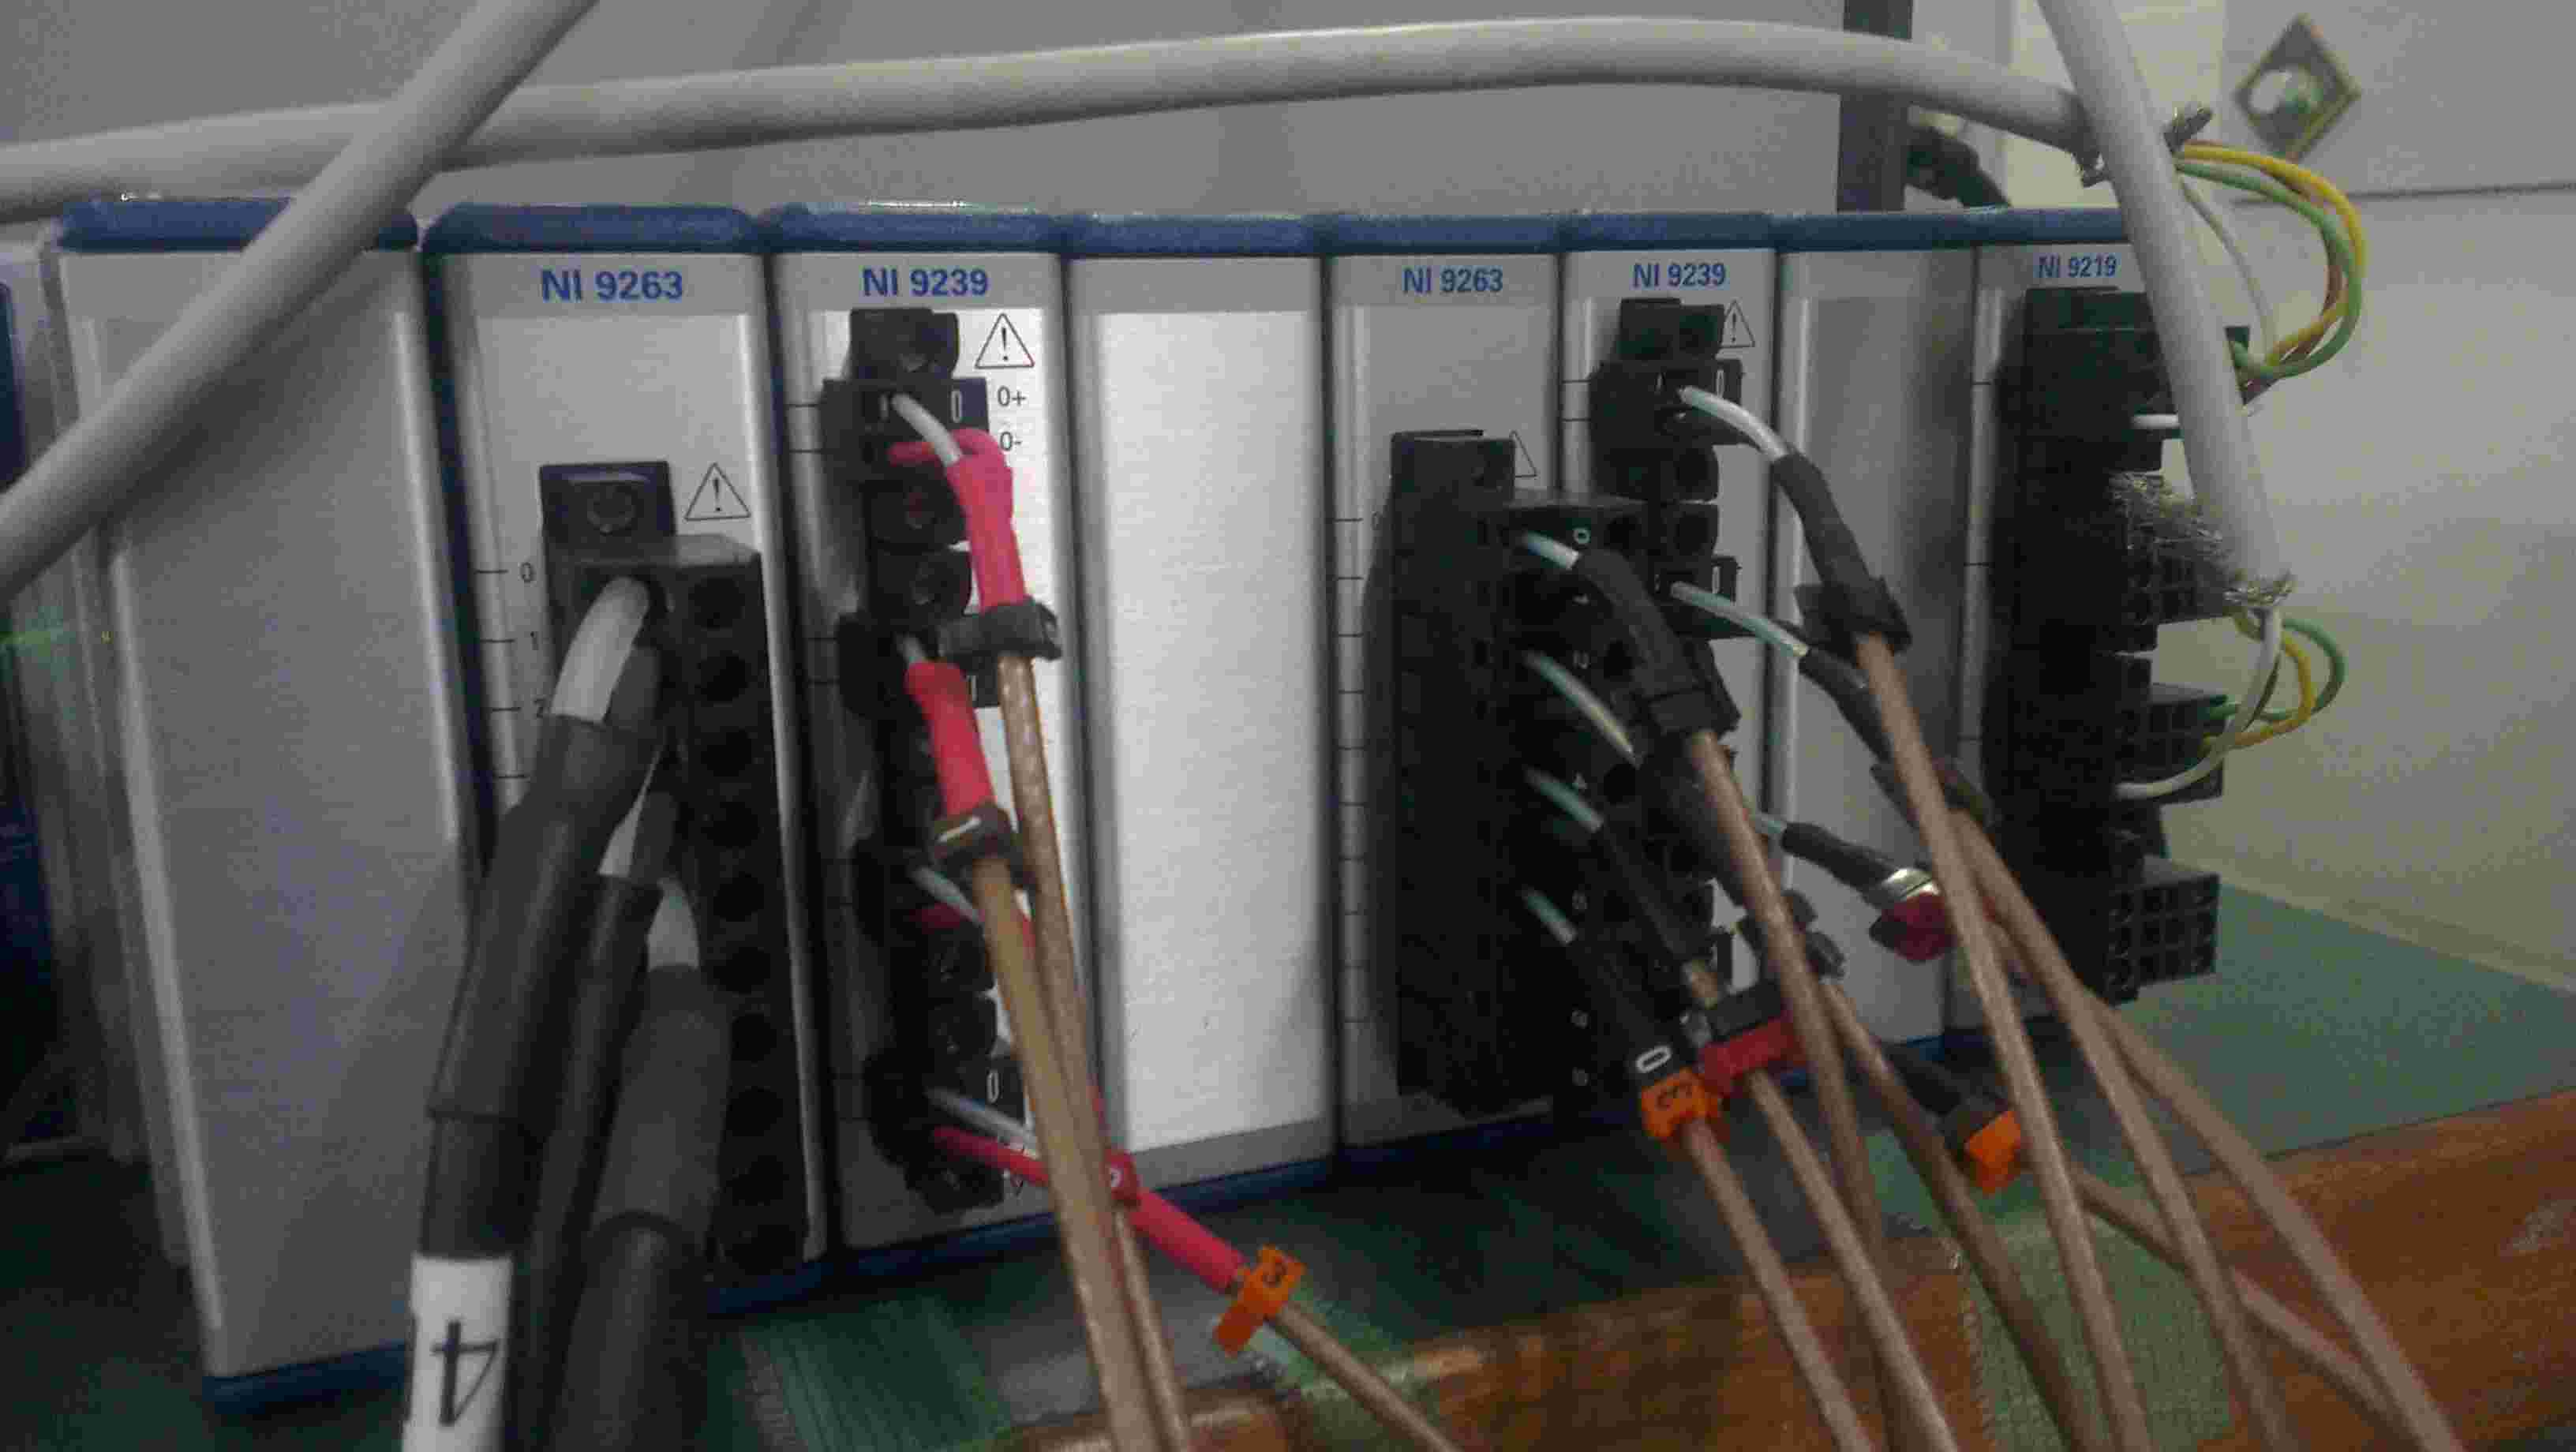
\includegraphics[height=2.5cm,width=6.2cm,angle=180]{ima06a.jpg}};
% %   \pause
%   \node (img4) at (4.4,1.0) {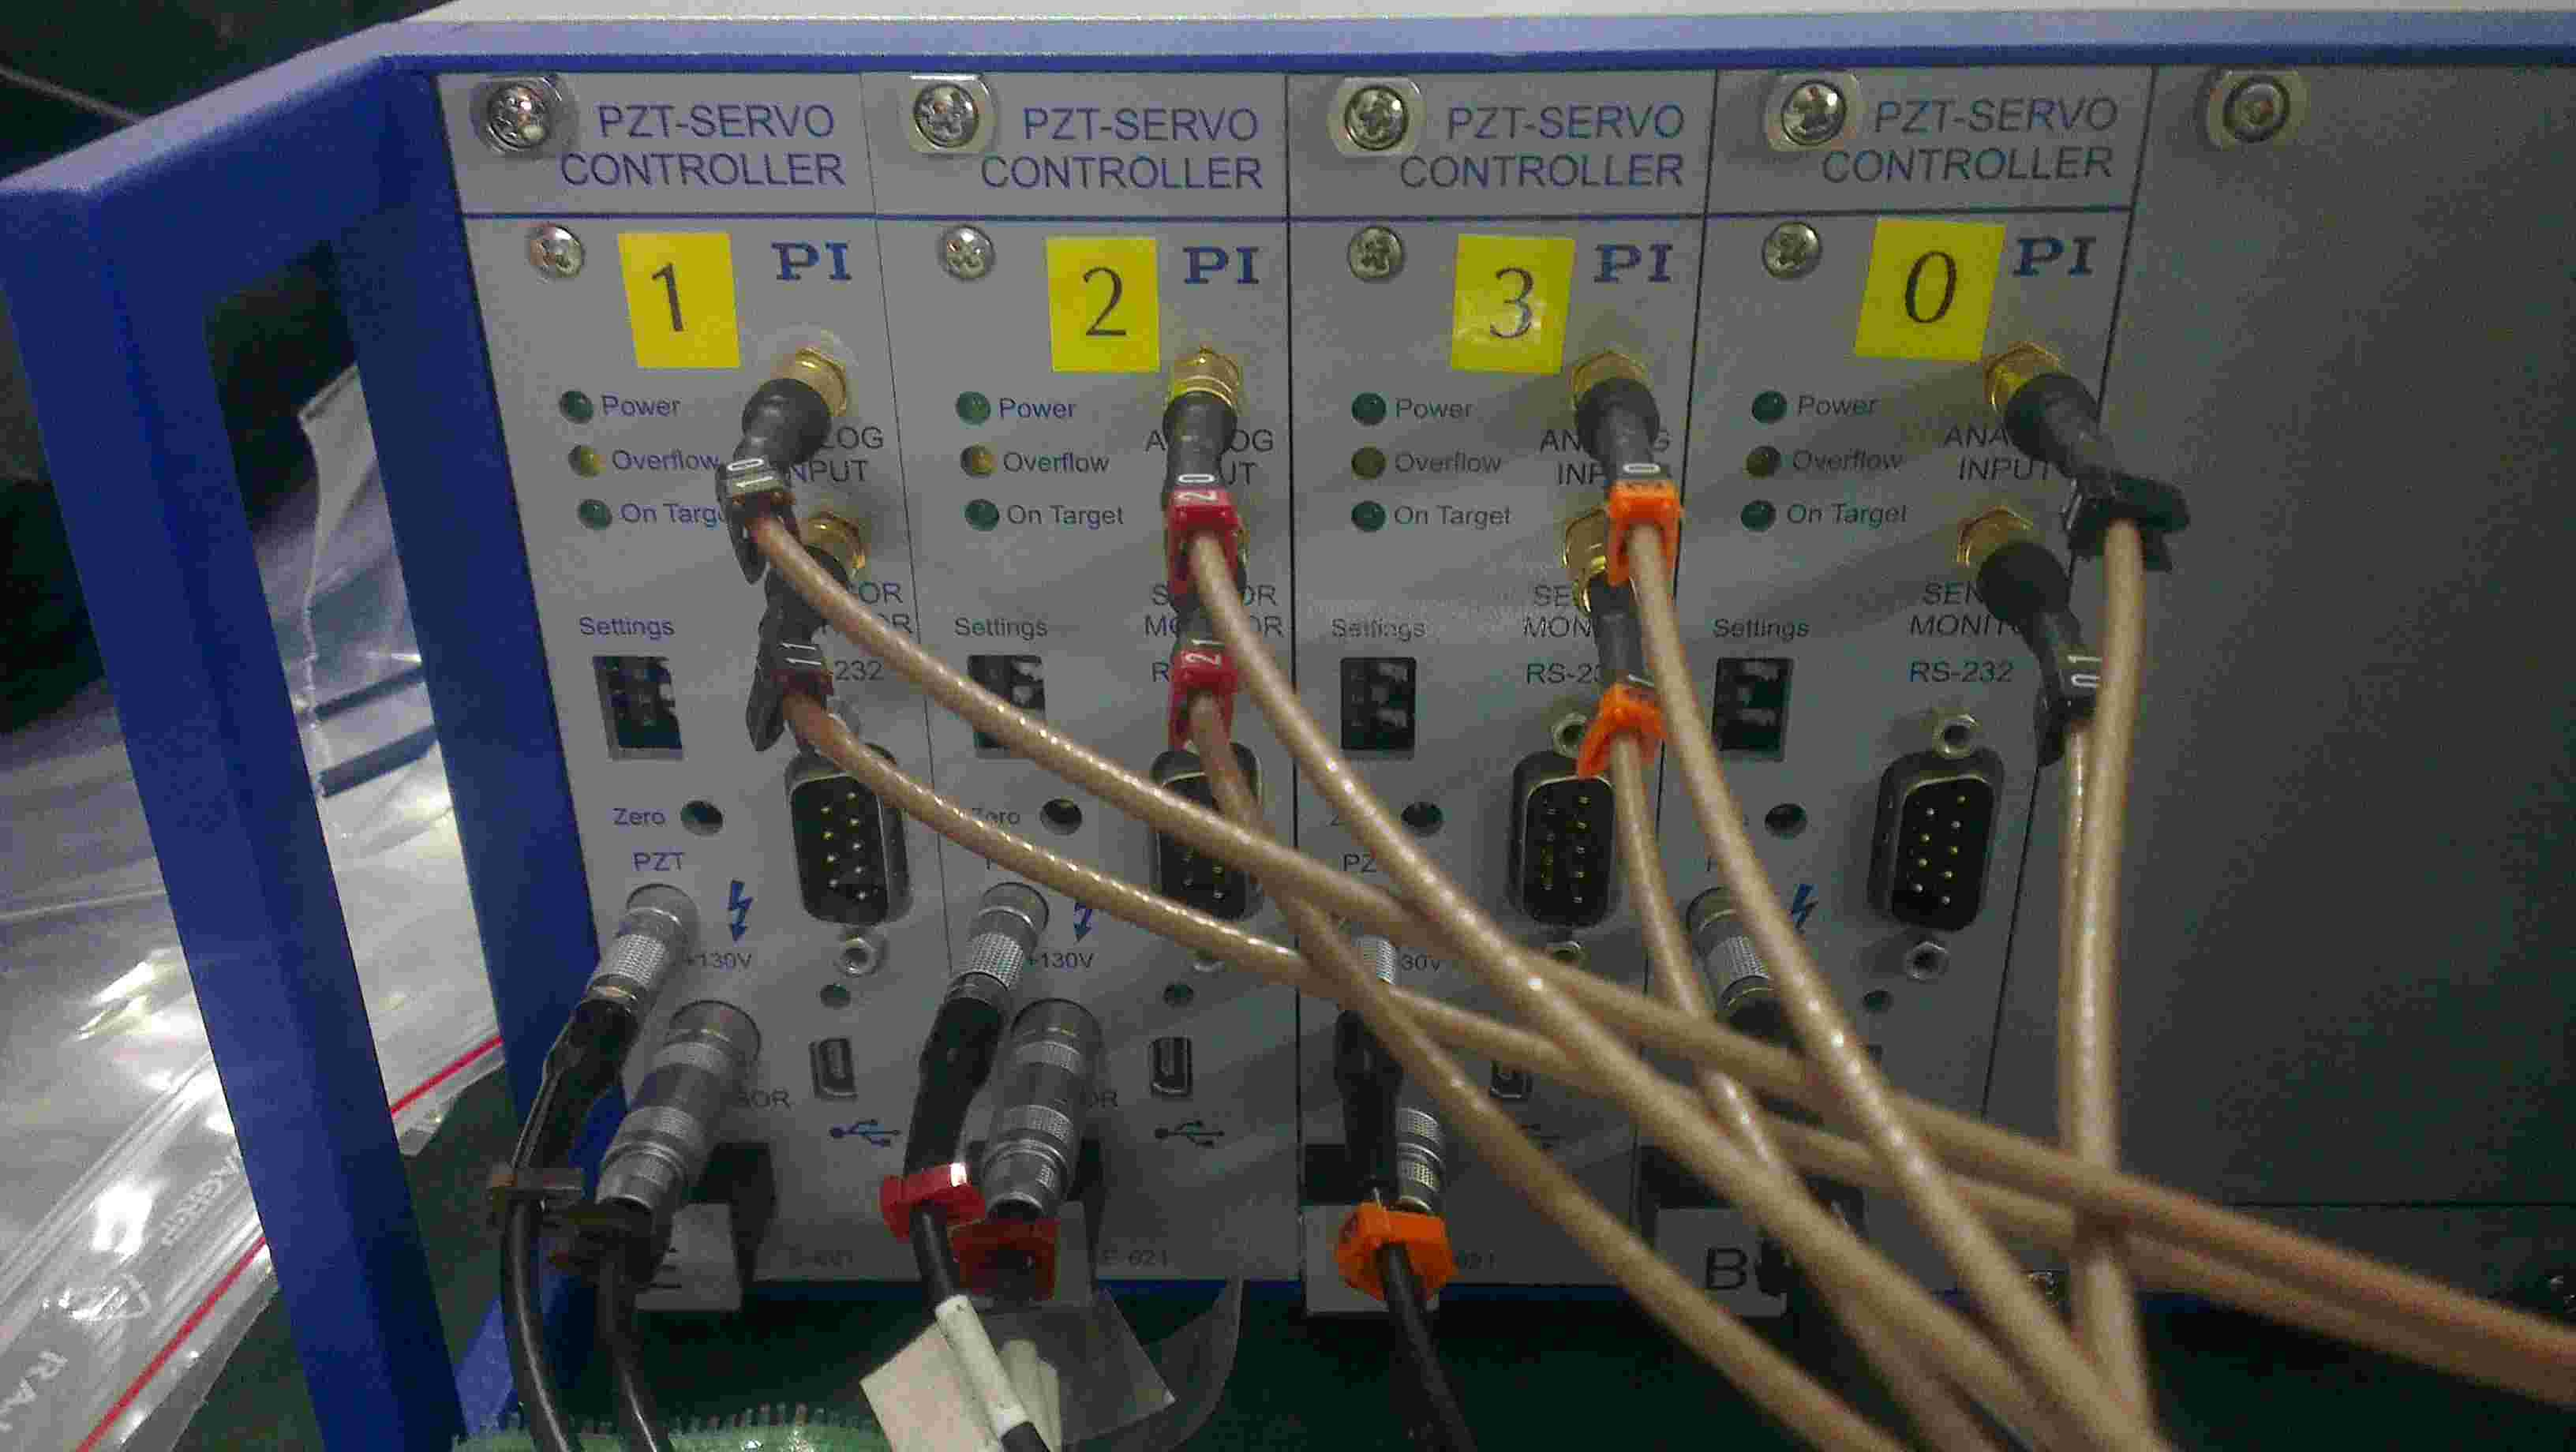
\includegraphics[height=1.6cm,width=3cm,angle=0]{ima04a.jpg}};
%   \node (img5) at (2.0,0.0) {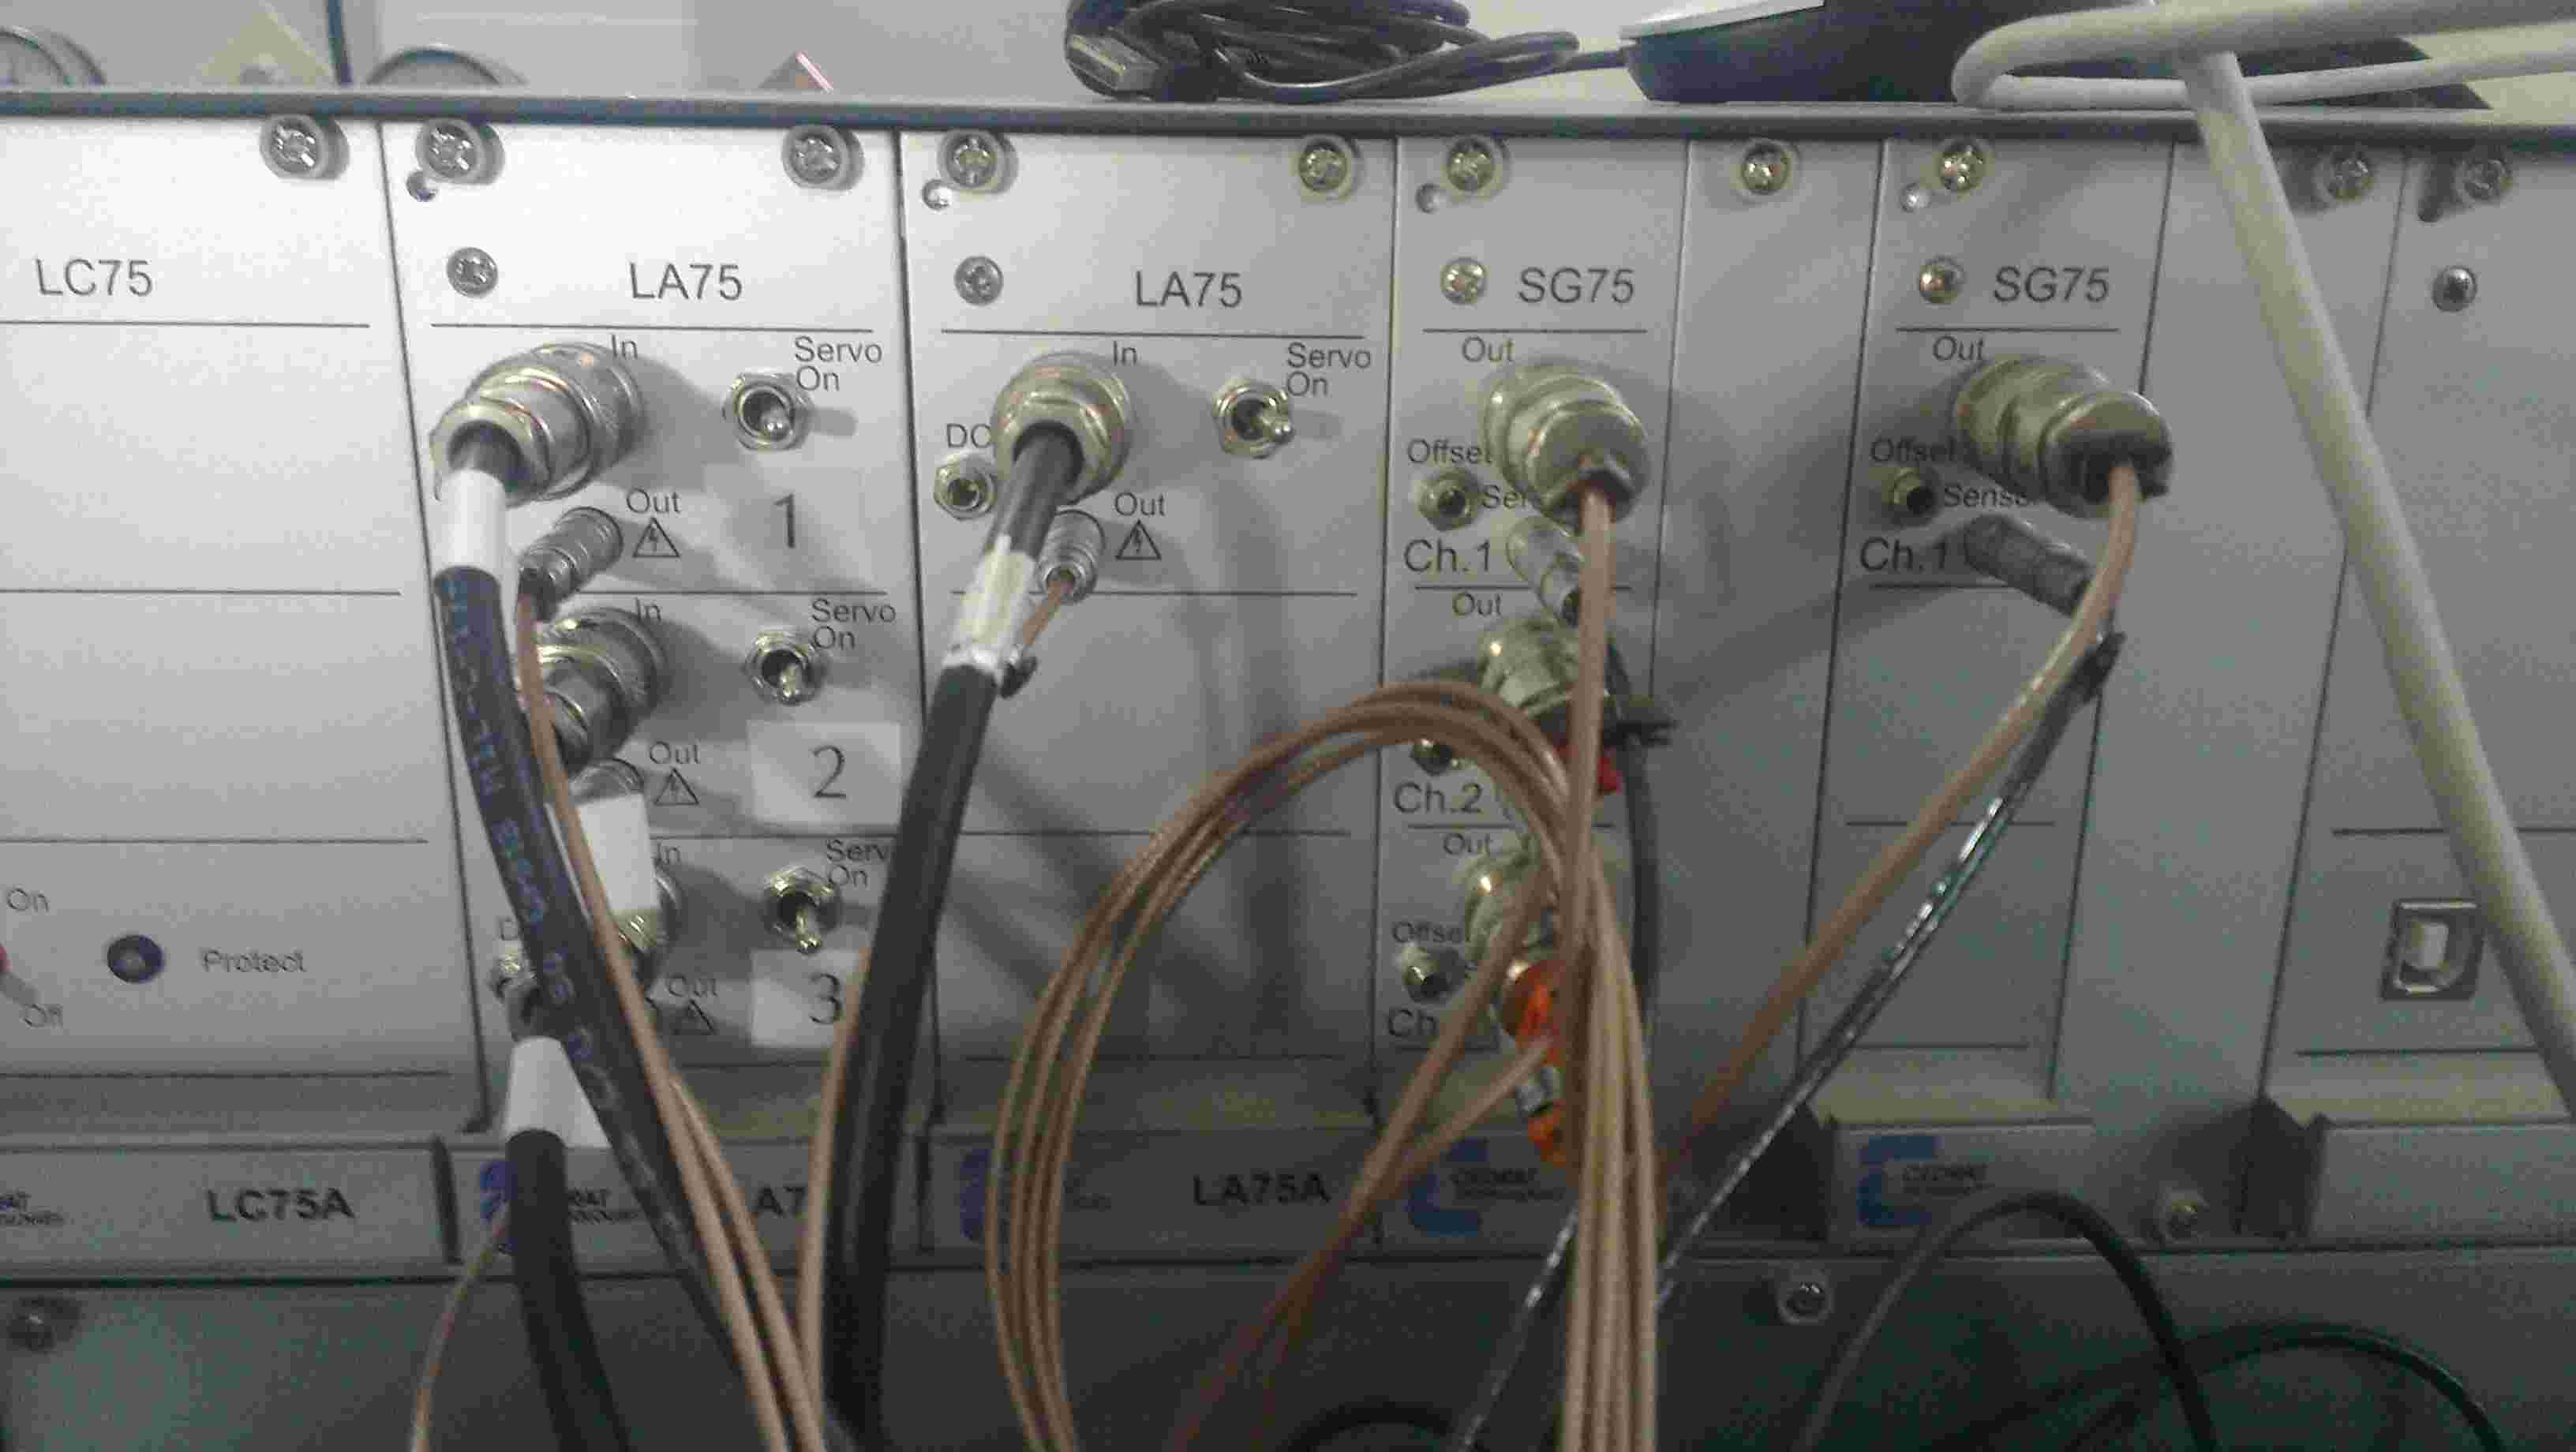
\includegraphics[height=1.6cm,width=3cm,angle=0]{ima05a.jpg}};
% %   \pause
%   \node (img6) at (4.4,3.0) {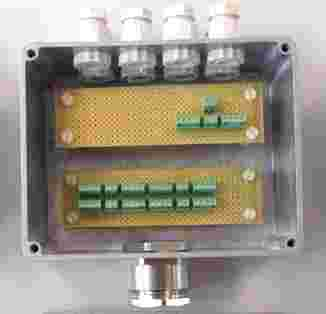
\includegraphics[height=1.6cm,width=3cm,angle=180]{ima08a.jpg}};
%   \node (img7) at (1.8,1.4) {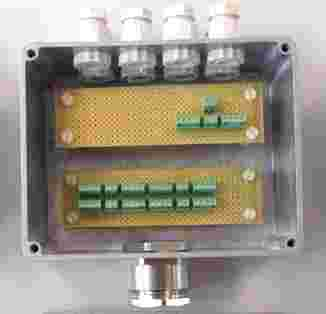
\includegraphics[height=1.6cm,width=3cm,angle=180]{ima08a.jpg}};
%   \node (img8) at (1.8,3.0) {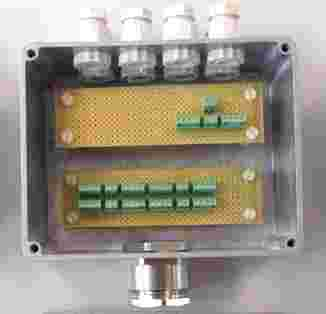
\includegraphics[height=1.6cm,width=3cm,angle=180]{ima08a.jpg}};
% %   \pause
%   \node (img9) at (-3.0,0.7)  {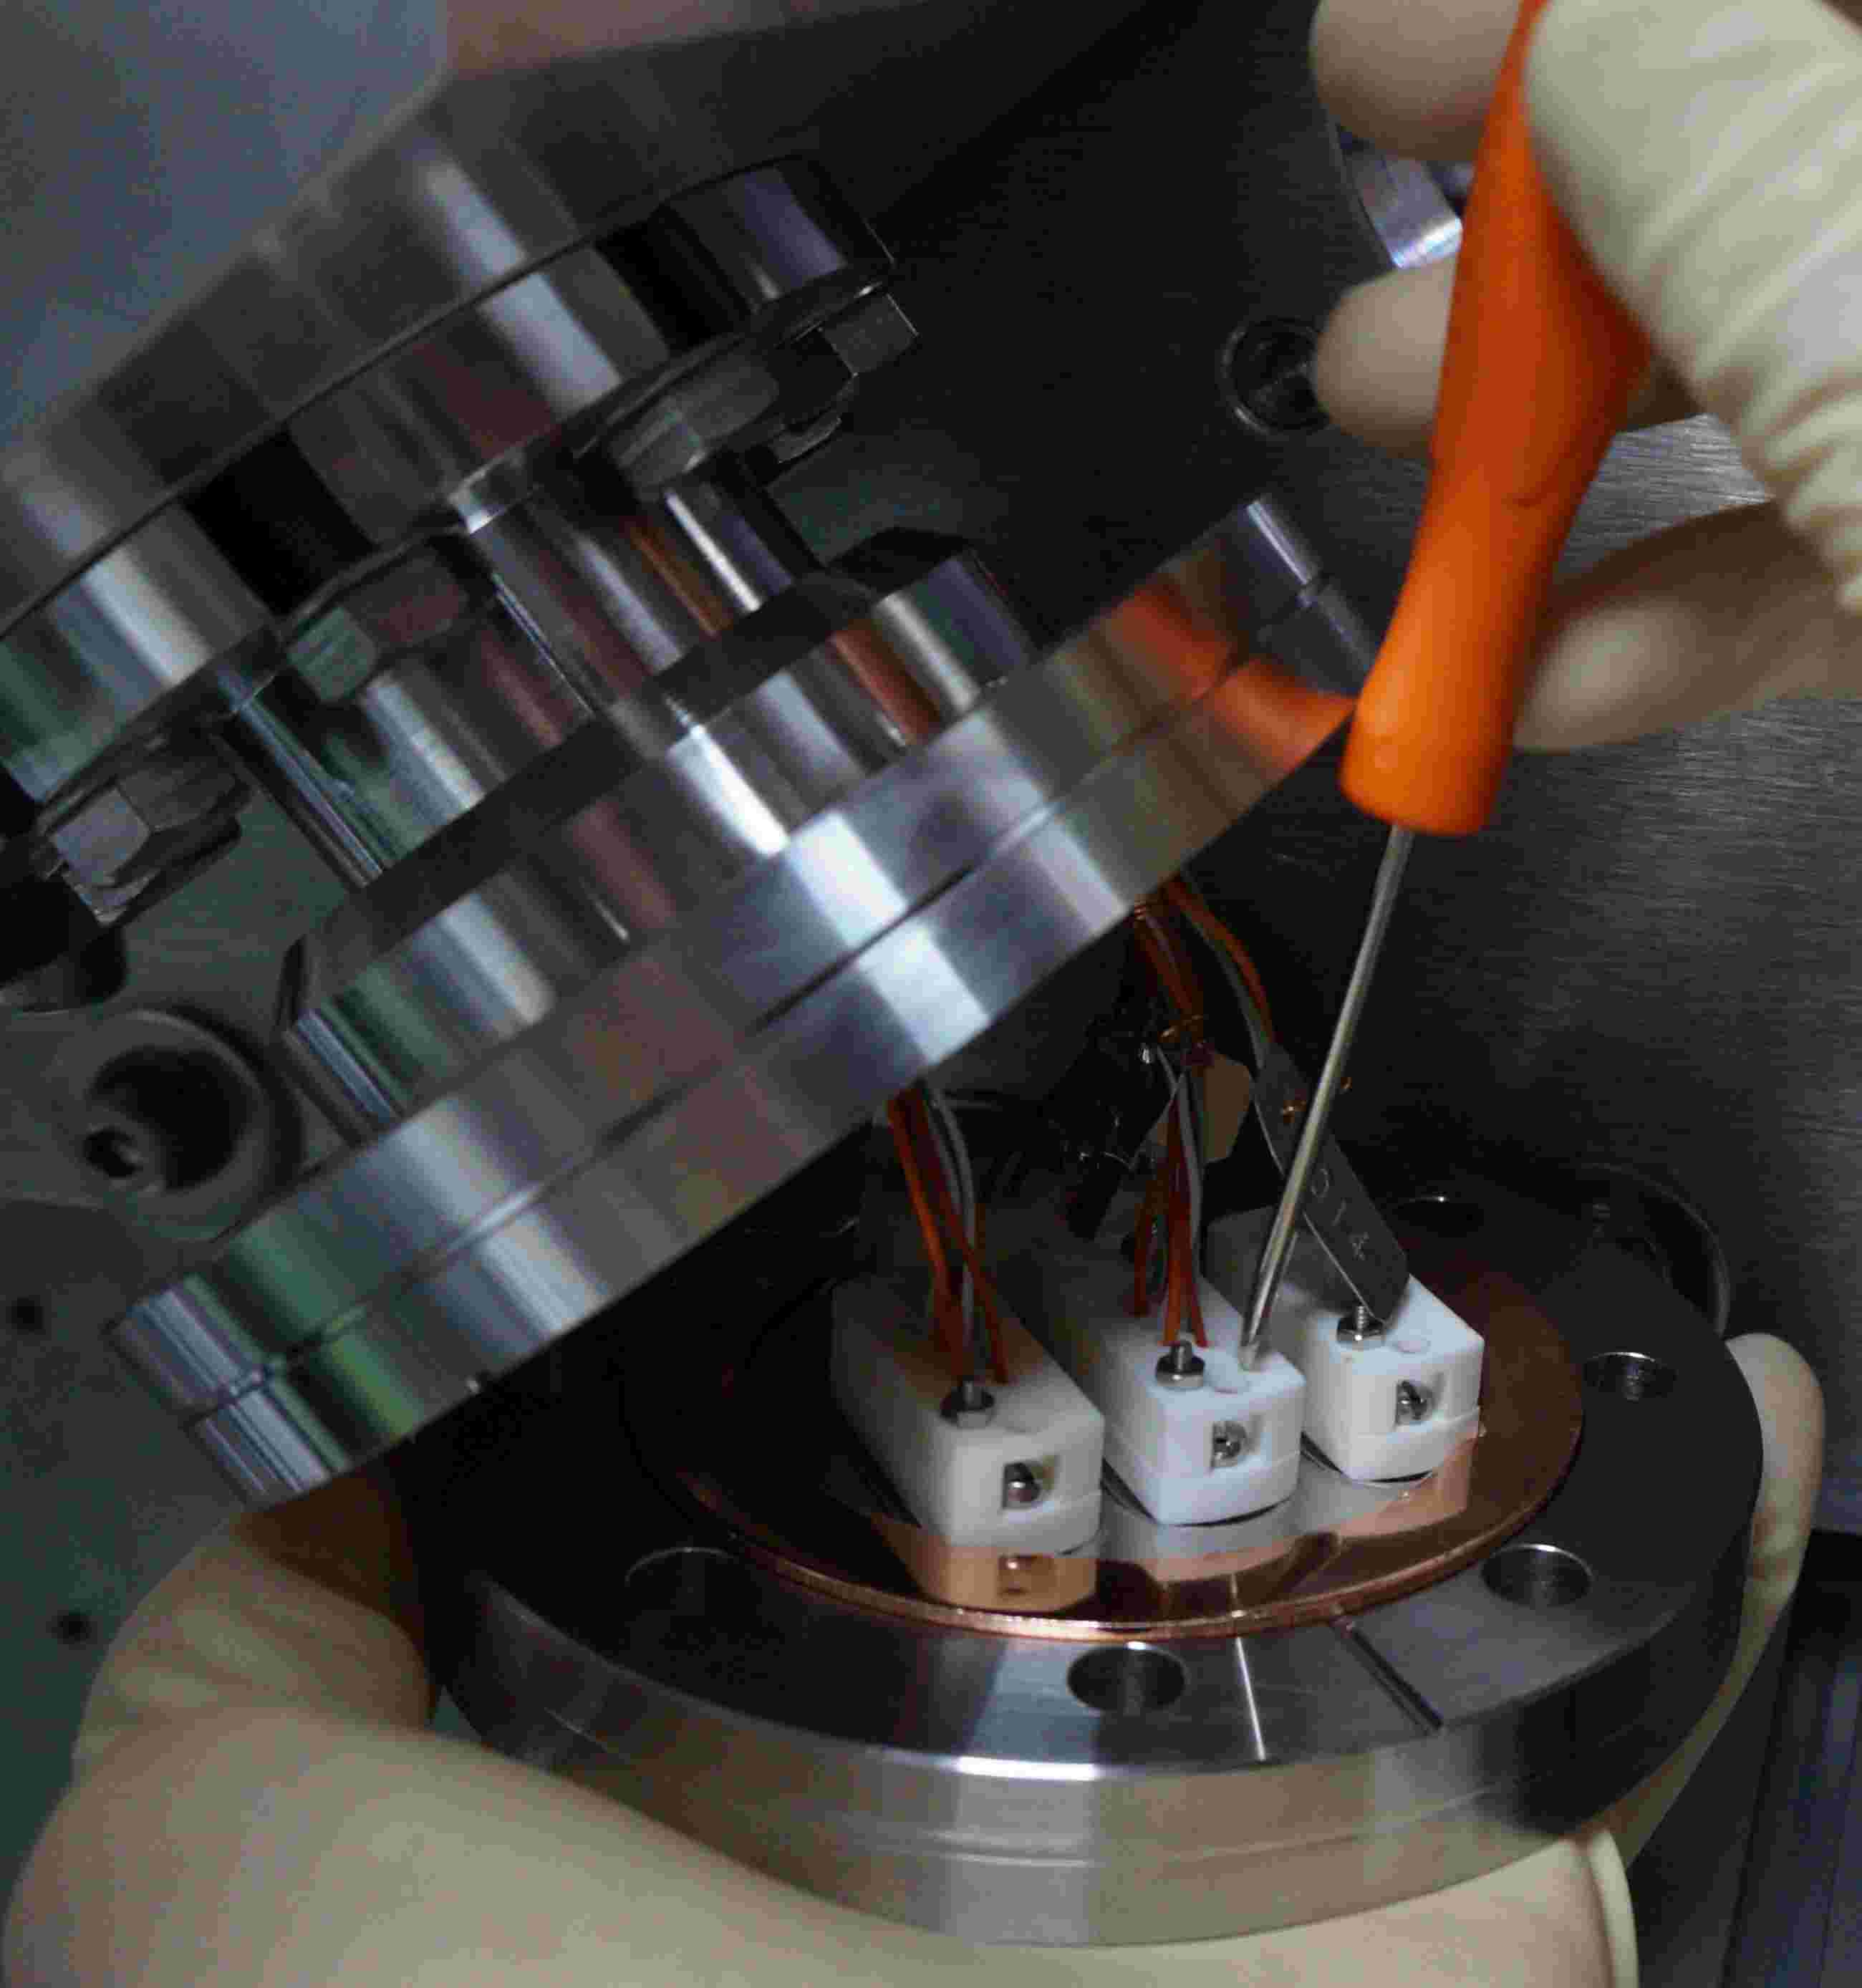
\includegraphics[height=1.6cm,width=1.4cm,angle=0]{ima10a.jpg}};
%   \node (img10) at (-3.0,3.0) {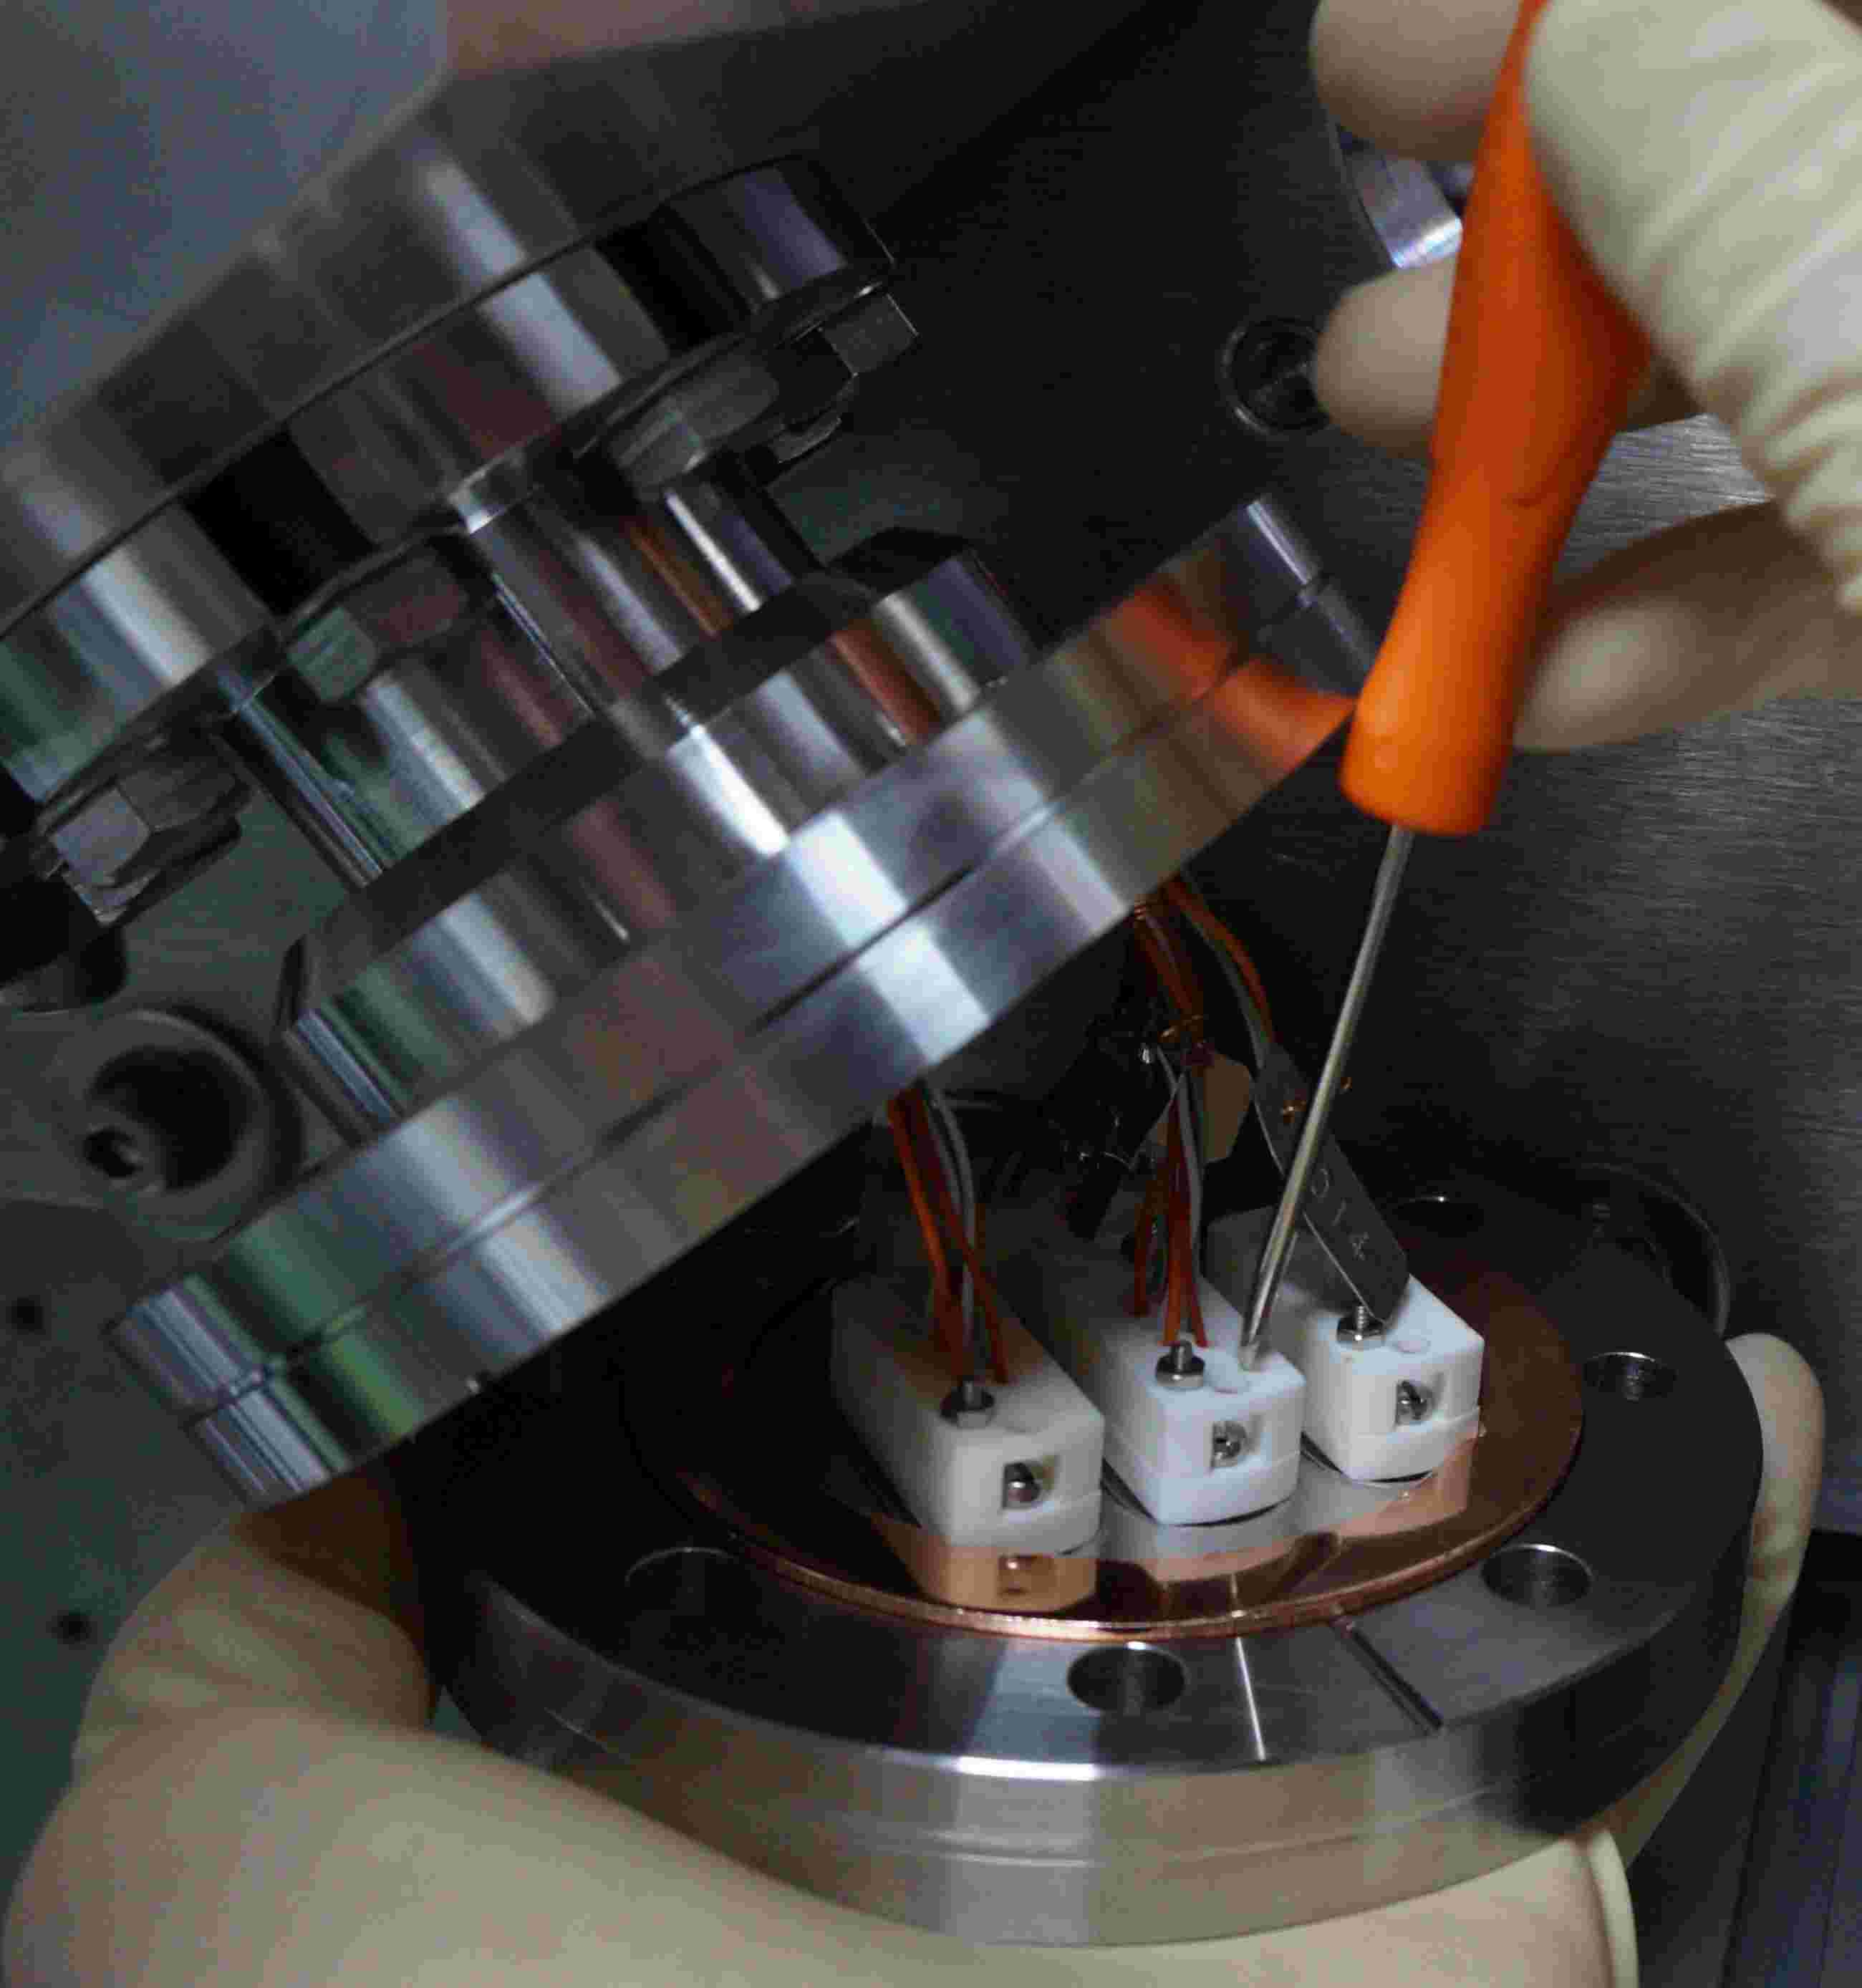
\includegraphics[height=1.6cm,width=1.4cm,angle=0]{ima10a.jpg}};
% %   \pause
%   \node (img11) at (-4.8,0.7)  {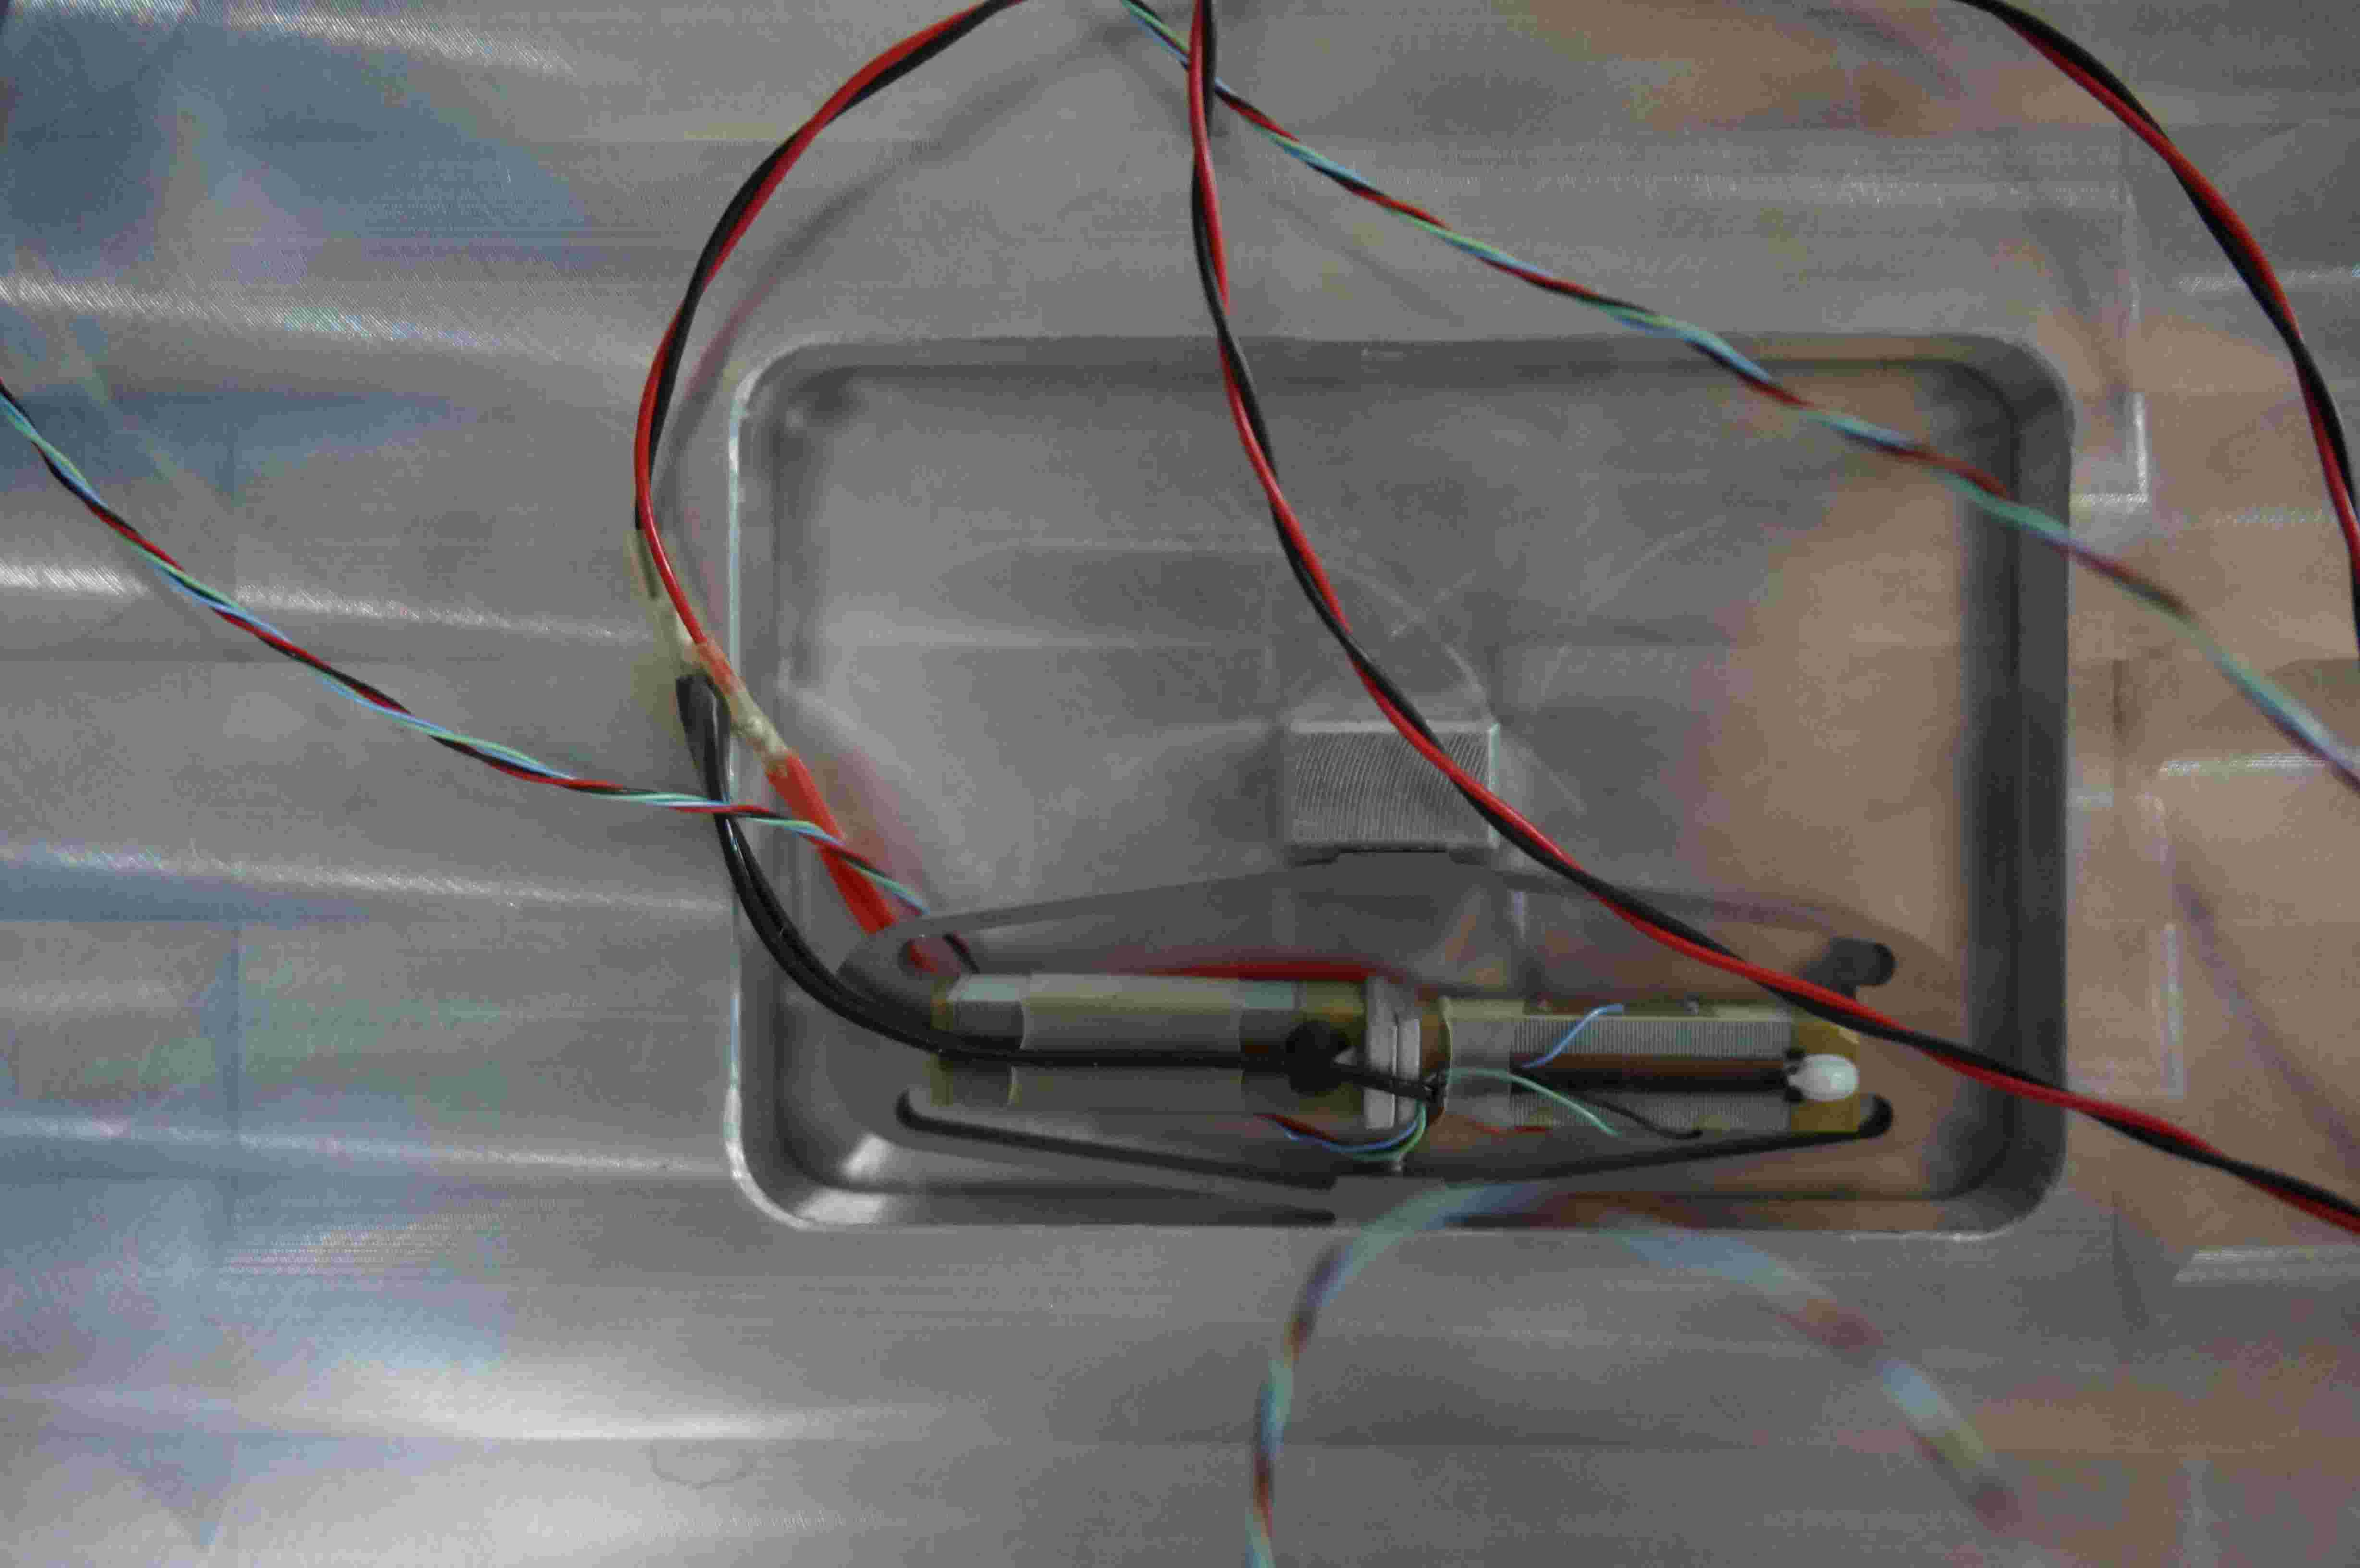
\includegraphics[height=1.6cm,width=1.4cm,angle=0]{ima11a.jpg}};
%   \node (img12) at (-4.8,3.0) {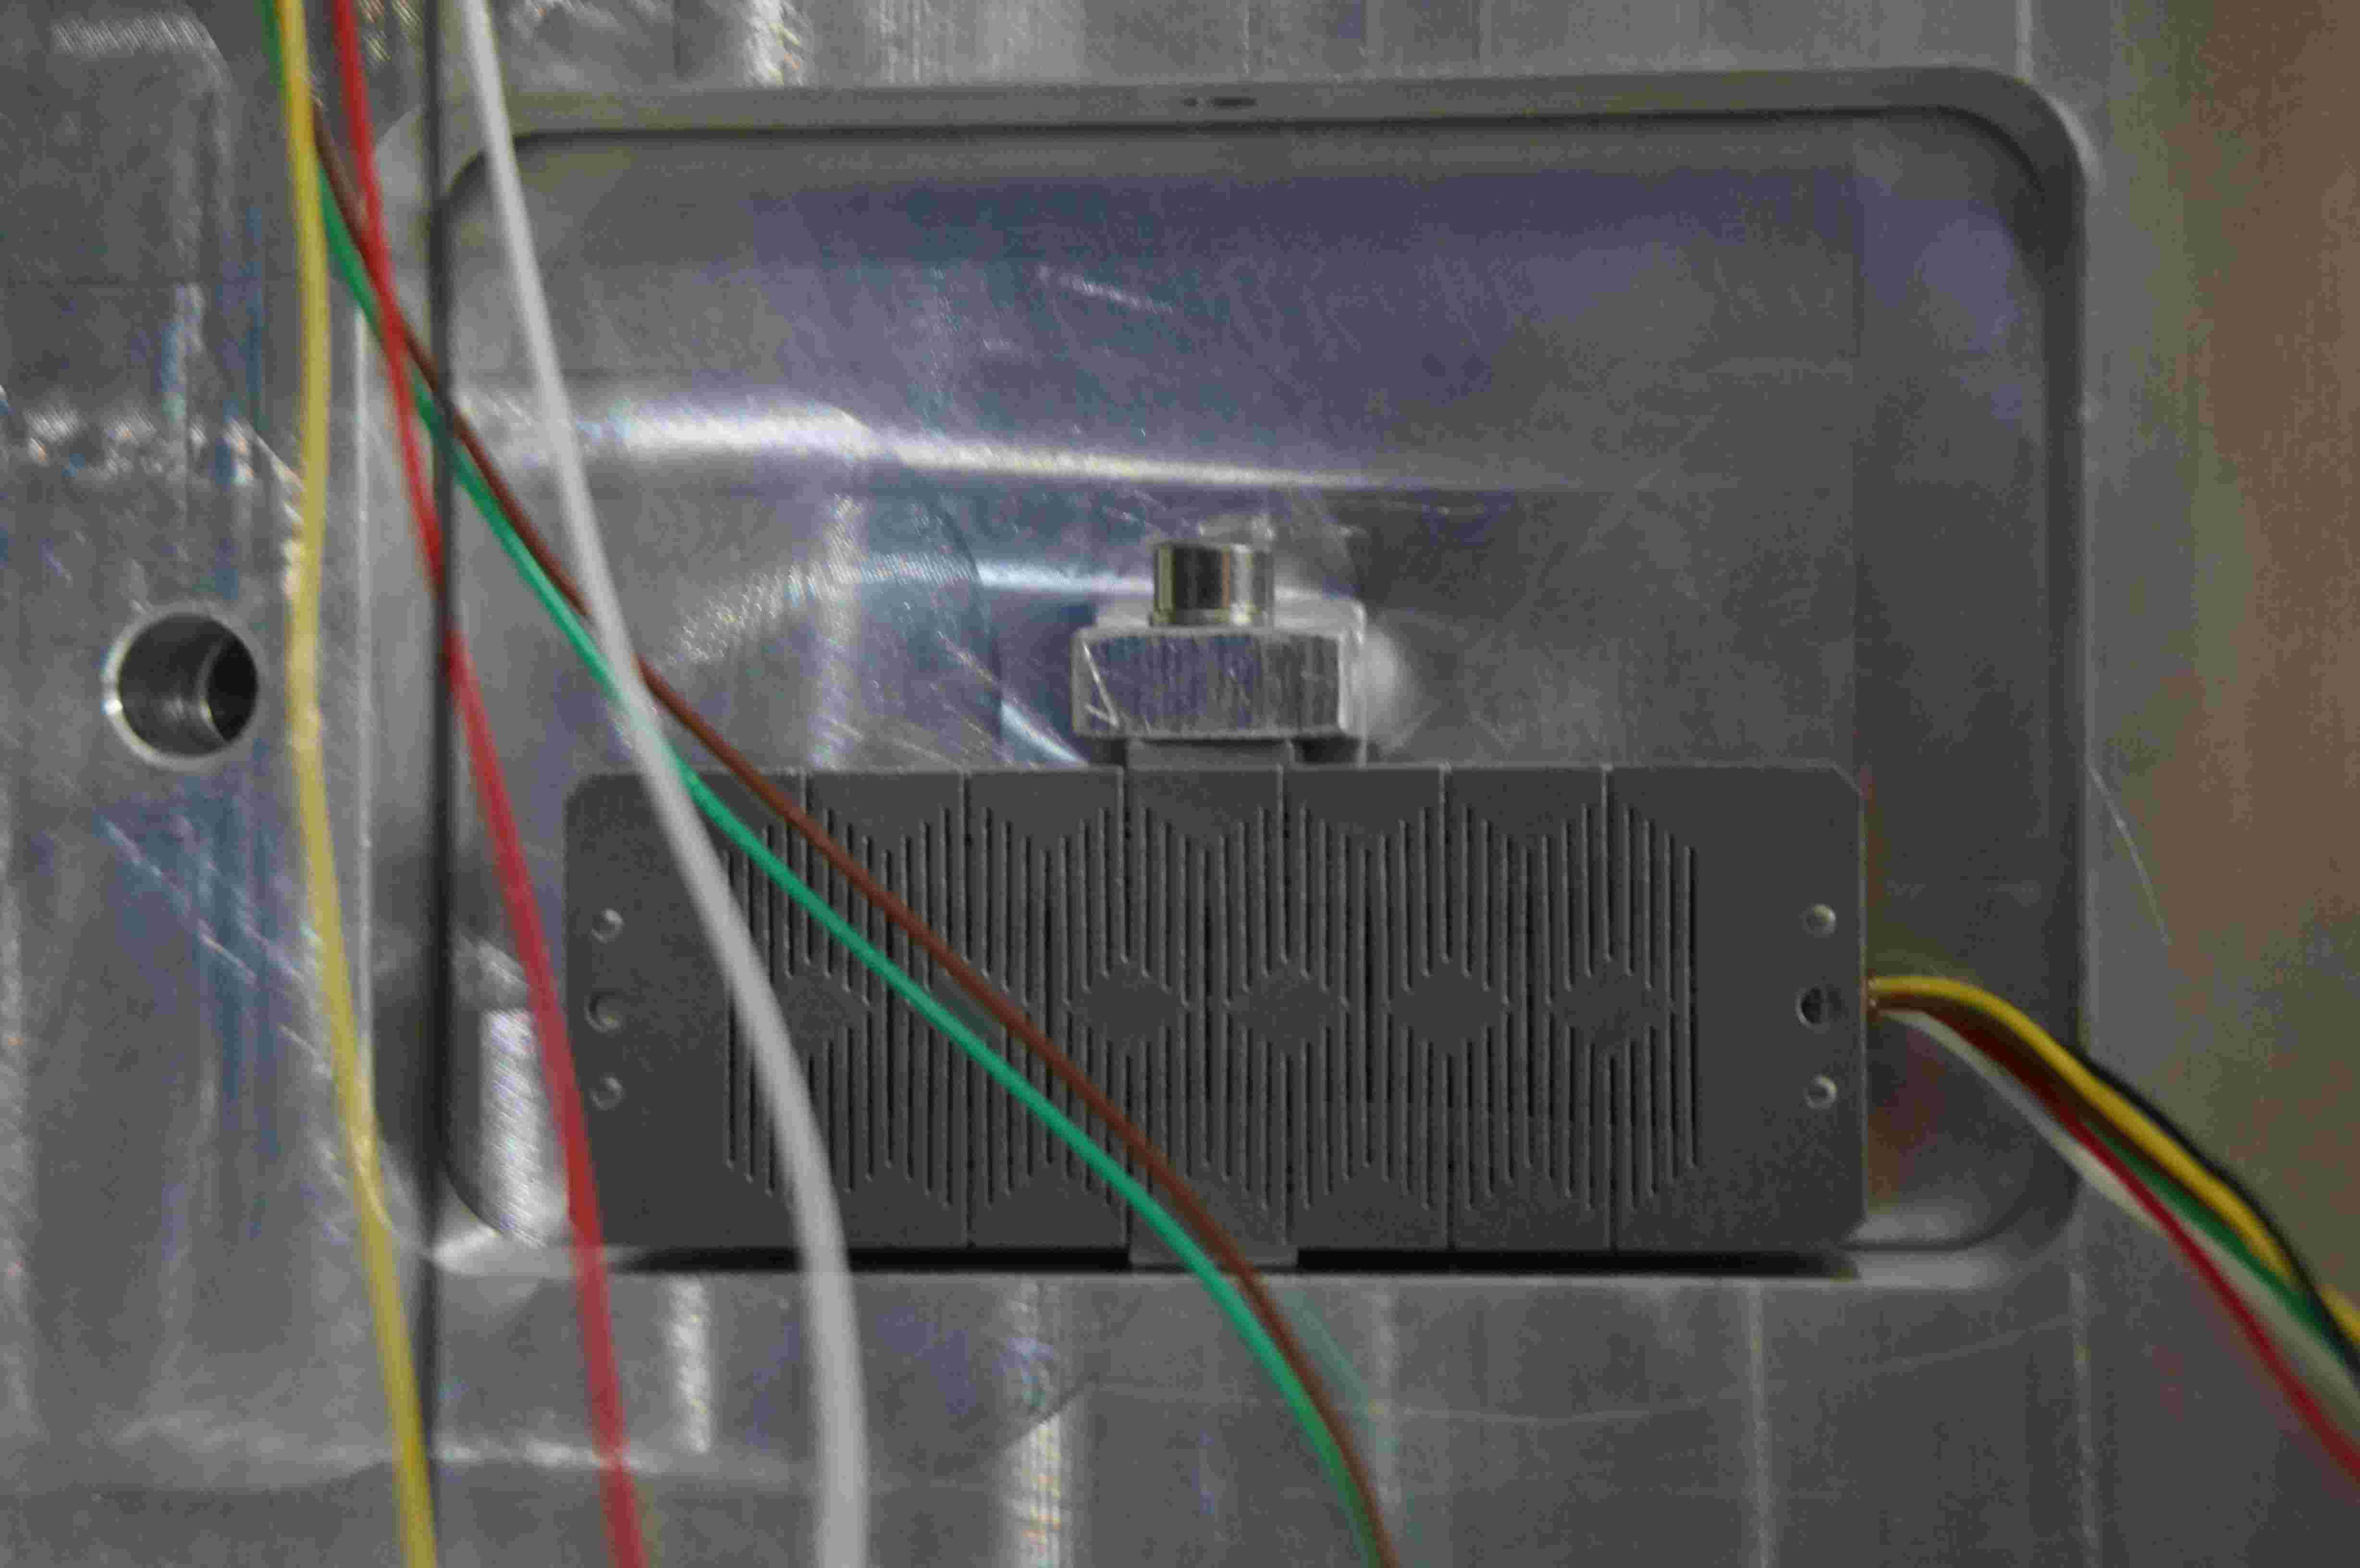
\includegraphics[height=1.6cm,width=1.4cm,angle=0]{ima12a.jpg}};
% \end{tikzpicture}\caption{Images from installation.}\label{f:imaginsta}
% \end{figure}
\subsubsection{Mover range}
PI and Cedrat have different ranges: PI~300~$\mu$m, Cedrat~250~$\mu$m. The Control voltage and displacement (min-max positions) is opposite between companies:\par
\begin{itemize}
\item PI: (min) 0~V to (max) 10~V
\item CEDRAT: (max) -1~V to (min) 7~V
\end{itemize}
It is important to note that:
\begin{itemize}
\item The voltage-displacement relation is inverse for CEDRAT movers.
\item When the system is OFF (0~V), PI mover are at its minimum, however CEDRAT are not.
\end{itemize}
\subsubsection{Mover Control}
Figure \ref{f:movercontrol} shows an schematic of the control system per mover. The voltage value is set via an EPICS Process Variable (PV), and it is send to a DAC, the analog voltage set the control box to move the piezo-electric. The displacement is measure by a set of strain-gauges. The FB loop is closed at the Control box. A read-out voltage is taken by the ADC and publish as another PV.\par
\begin{figure}[hbt]
\centering
\begin{tikzpicture}
 \node (img1) {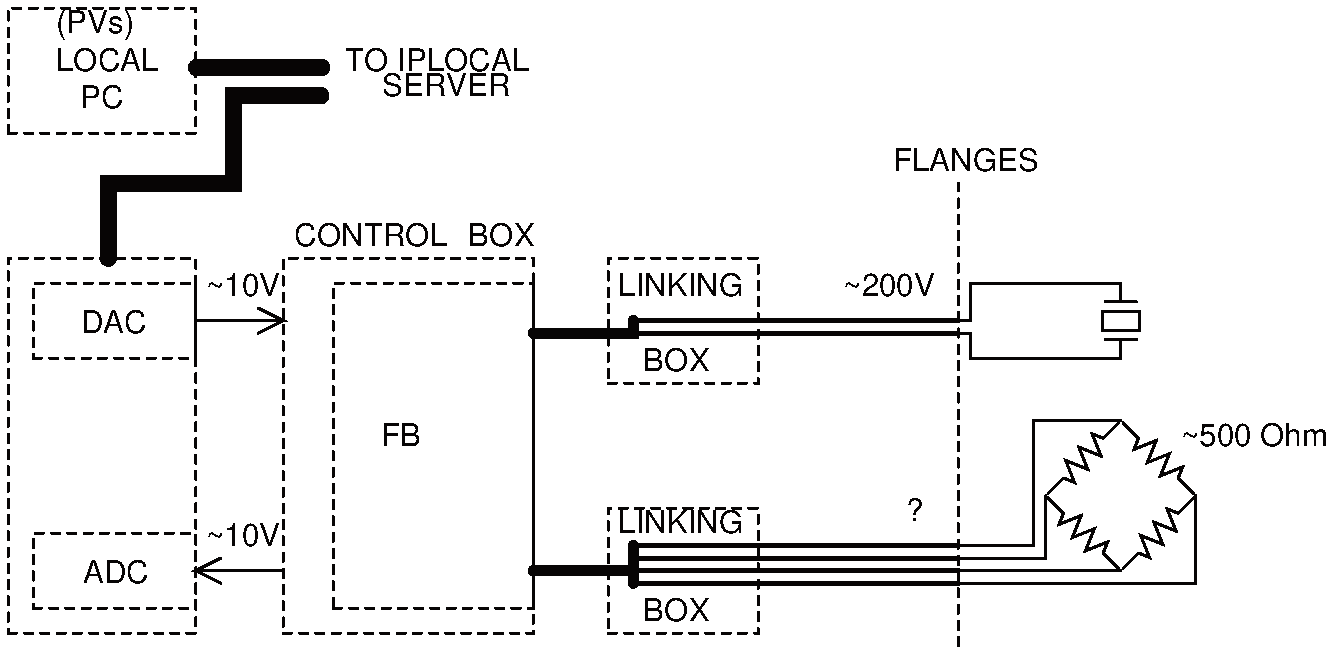
\includegraphics[scale=0.5]{Page1.pdf}};
 %\node (img2) at (4.4,1.5) {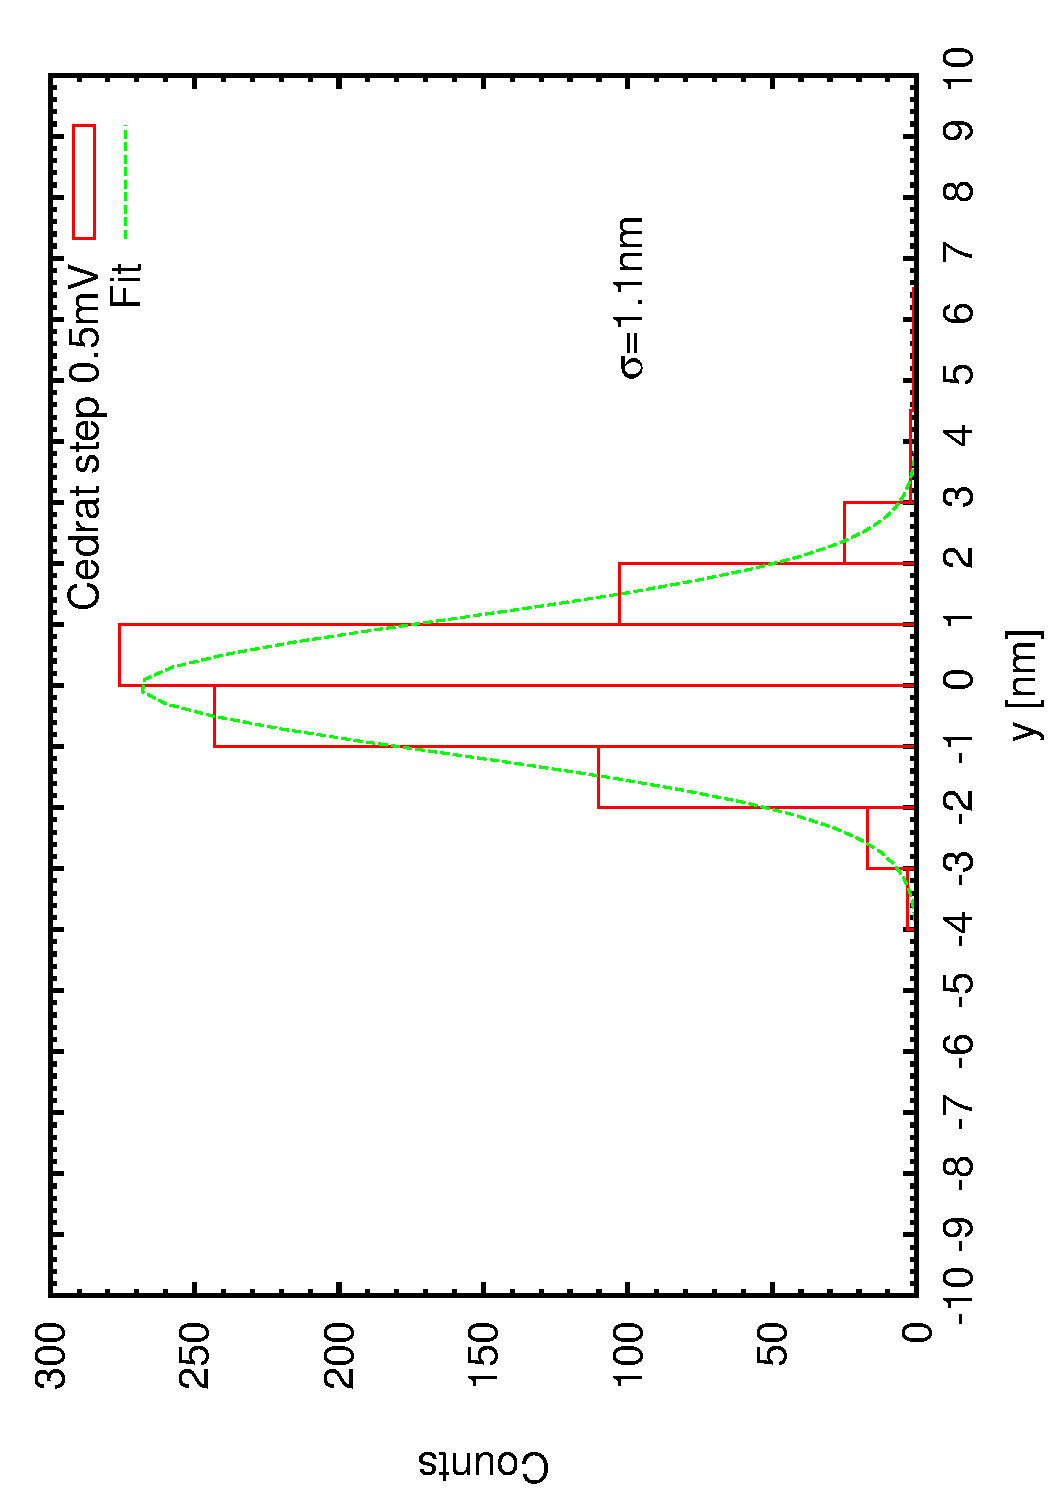
\includegraphics[scale=0.1,angle=-90]{imagestep12.pdf}};
%  \node (img3) at (4.4,2.6) {$\sigma_y=$?};
 %\node (img3) at (4.4,1.5) {{\LARGE\color{red} ?}};
\end{tikzpicture}\caption{Control system per mover.}\label{f:movercontrol}
\end{figure}
% The DAC setpoints used:BLOCK AB 1~mV=31.25~nm, BLOCK C 1~mV=30~nm\par
\subsubsection{Feedback and NO Feedback}
There are two operation possibilities per mover: Feedback (fb) and No Feedback (no fb). It means 8 feedback loops. On each case the control module sets a voltage value on the mover and read the strain gauge to create a closed loop. However, their implementations are different on each company.
\subsection{The PLC}
Two NI9263 are used to set analogue voltage into the mover control electronics. Two NI9239 are used to read analogue voltage from the strain gauge readback. One NI9219 is used to read temperature. These modules are connected to the chassis NI9188 which is connected by network to a working station with Labview installed.
The block chassis+NI modules is called \textbf{PLC}.\par
\textbf{National instruments Chassis: NI9188}
\begin{itemize}
\item Mac Address: 0080.2f14.b777
\item DHCP
\item IP address (ATF) 31.1.1.39
\item IP address (KEK): None
\item Host name: ipmv-plc.ip-local
\item Net Mask: 255.255.255.0
\item connected to ip-local during installation
\end{itemize}
Chassis NI9188 can connect up to 8 modules, not all are used:
\begin{itemize}
\item PI
\begin{itemize}
\item Module 5: NI9263 Digital to analogue converter
\item Module 6: NI9239 Analogue to digital converter
\end{itemize}
\item Cedrat
\begin{itemize}
\item Module 2: NI9263 Digital to analogue converter
\item Module 3: NI9239 Analogue to digital converter
\end{itemize}
\item Temperature
\begin{itemize}
\item Module 8: NI9219 Temperature probes
\begin{itemize}
\item Cedrat: 	Channel 0
\item PI: Channel 2
\end{itemize}
\end{itemize}
\item The other slots are not used
\end{itemize}
\subsection{The PC}
It is used to control from close locations the BPM positioning system. It sets the digital values to put in the PLC and reads the digital values from the PLC channels corresponding to strain gauges.\par
\subsubsection{Characteristics}
LAL Computer (Laptop)
Processor Inter Core i7 vPro\par
Mac Address: d067.e550.620e\par
\subsubsection{Network Parameters}
DHCP\par
IP address(ATF): (31.1.1.38) ipmover-pc.ip-local\par
Net Mask: 255.255.255.0\par
Connected to ip-local server\par
\subsubsection{Used Software}
Windows 7 Francais\par
National Instrument - Labview 2011\par
National Instruments - Measurement $\&$ Automation Explorer (NI MAX) 5.4\par
Evince 2.32.0\par
CALab (Labview + EPICS) \cite{CALab}\par
% In adition, this Software is present but not used by movers:\par
% SIOS Interferometer Software INfasNTC 6.3.1.42 2012\par
% Festo Positioning Drivers\par
% \subsubsection{Access}
% Account (Nom d'utilisateur): *******\par
% % Connect to (Se connecter \'a): NB\_SALLE101 (cet ordinateur)\par
% Password: KEKJapan2012\par
\subsubsection{Folder Content Description}\par
Path to applications and info\par
\verb?Bureau/Actionneurs Piezo/Applis?\par
All applications were done in Labview. Filenames give an indication of its purpose, here are some keywords used in filenames:\par
\begin{itemize}
\item \verb?oscilloscope?: uses de ADC to read signals
\item \verb?generateur?: function generator, uses de DACs to produce signals
\item \verb?Actionneurs positionnement BPMs?: activate the system displacement
\item \verb?Ethernet?: connected by wired network,
\item \verb?USB?: corresponds to previous version connected by USB.
\item \verb?Verticaux groupe?: all 3 vertical mover movers are activated by one only setting.
\item \verb?mouvements identiques?: first version of BPM displacement system (PI and CEDRAT) integrated.
\item \verb?Jauges?: stores the strain gauges info in excel format.
\item \verb?temp?: stores the strain gauges and temperature info in excel format.
\item \verb?epics?: control from epics system, Labview works as interface.
\item \verb?Actionneurs multicycles?: several cycles over the defined voltage range are performed
\item \verb?Cedrat, PI?: identifies the group of movers to use.
\item \verb?Vertical, lateral fixe?: it means that one direction of movement is set (fixed) to a voltage value while the other direction varies in cycles.
\end{itemize}
\subsubsection{PVs}
Epics PVs (Process Variables). Write: sets a value on the DAC. Read: reads from ADC.\par
Channels IP:BPM-AB:Mover0 and IP:BPM-C:MoverB are for lateral movement.\par
IP:BPM-AB:Mover0:Read\par
IP:BPM-AB:Mover0:Write\par
IP:BPM-AB:Mover1:Read\par
IP:BPM-AB:Mover1:Write\par
IP:BPM-AB:Mover2:Read\par
IP:BPM-AB:Mover2:Write\par
IP:BPM-AB:Mover3:Read\par
IP:BPM-AB:Mover3:Write\par 
IP:BPM-C:MoverB:Read\par 
IP:BPM-C:MoverB:Write\par 
IP:BPM-C:MoverC:Read\par 
IP:BPM-C:MoverC:Write\par 
IP:BPM-C:MoverD:Read\par 
IP:BPM-C:MoverD:Write\par 
IP:BPM-C:MoverE:Read\par 
IP:BPM-C:MoverE:Write\par 
IP:BPM-AB:Temp\par 
IP:BPM-C:Temp\par 

\section{The BPMs}\label{s:BPMscoord}
\subsection{Coordinate system}\par
Each BPM has its own coordinates with respect to a reference system centered electrically as in Fig.~\ref{f:BPMcoordinate}.\par
\begin{figure}[h]
\centering
  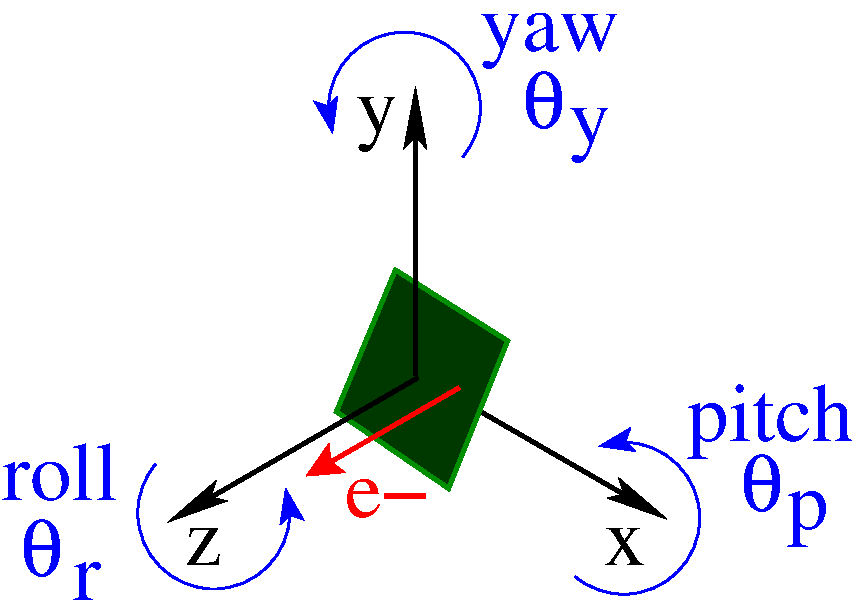
\includegraphics[scale=0.3,angle=0]{fig23.pdf}\caption{BPM coordinate system centered ellectrically. Beam in red, BPMs in green.}\label{f:BPMcoordinate}
\end{figure}
The coordinates of the beam and the BPM angle rotations are:
\begin{itemize}
 \item Beam Position: $x_A,y_A,z_A$, $x_B,y_B,z_B$, $x_C,y_C,z_C$
 \item BPM Angles respect to ref. system:  $\theta_{Ap},\theta_{Ar},\theta_{Ay}$, $\theta_{Bp},\theta_{Br},\theta_{By}$, $\theta_{Cp},\theta_{Cr},\theta_{Cy}$
\end{itemize}
All systems relate to a common mechanical reference system with no rotations, just translations in Fig.~\ref{f:ref3BPMs}. For simplification, one of the BPMs could be chosen to coincide with the common reference.\par
\begin{figure}[h]
\centering
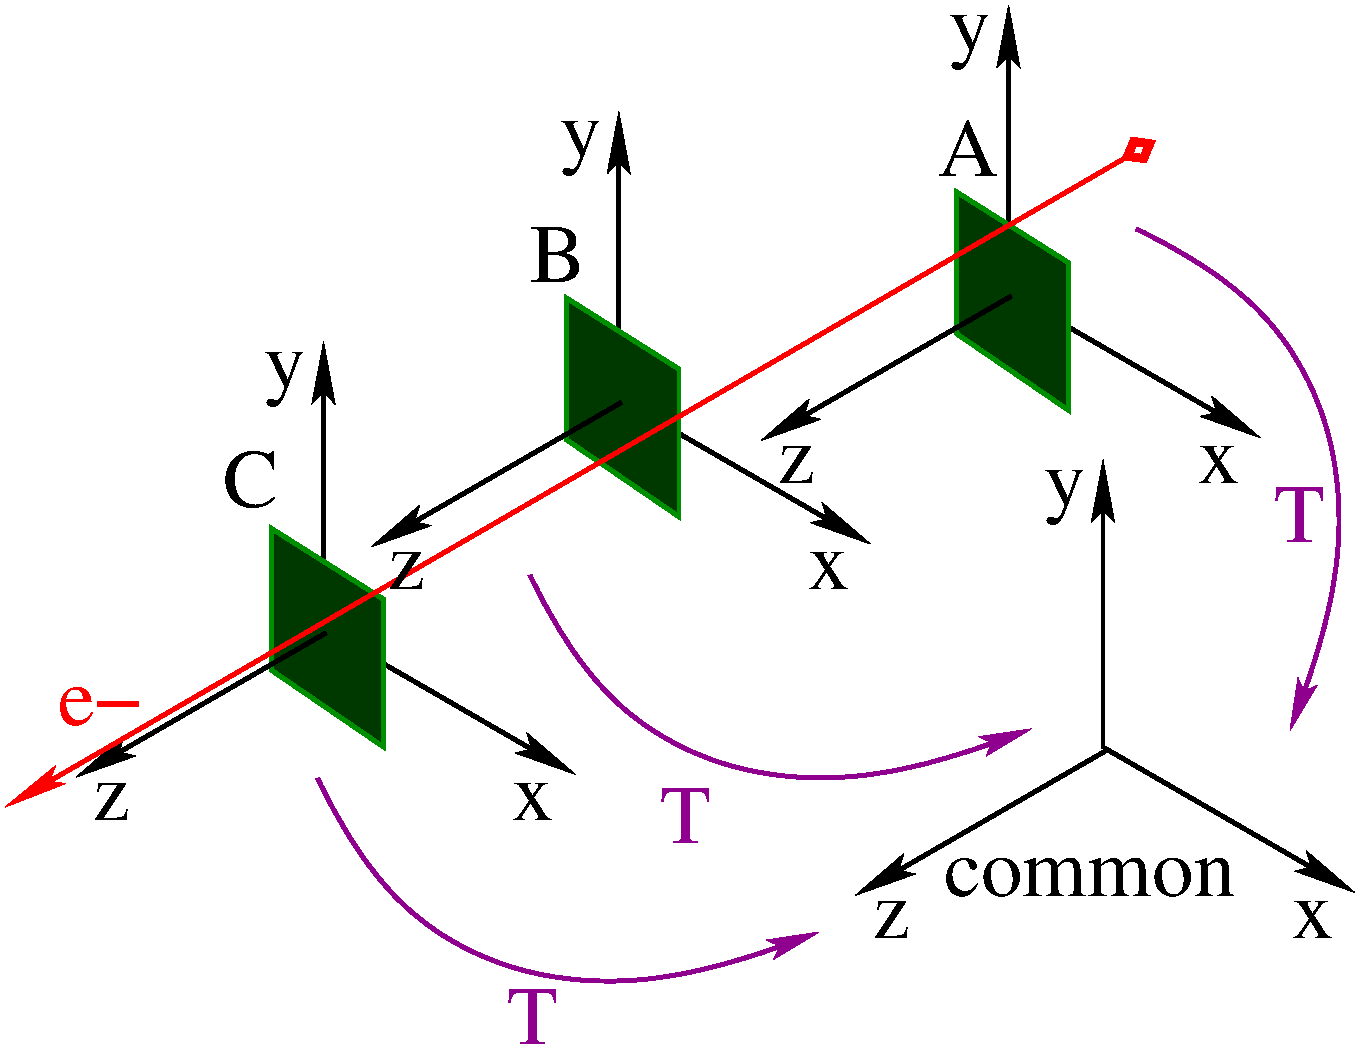
\includegraphics[scale=0.2,angle=0]{fig17.pdf}\caption{Reference system for the 3 BPMs.}\label{f:ref3BPMs}
\end{figure}
%\begin{columns}
%\begin{column}{3.5cm}
The set of movers to control BPM position is shown in Fig.~\ref{f:moverss}. This is expressed in Eq.~(\ref{eq:poscorr}) where during the installation all initial values (with 0-index) are set. A mover combination can change the transverse positions and the pitch angle per block.\par
\begin{figure}[h]
\centering
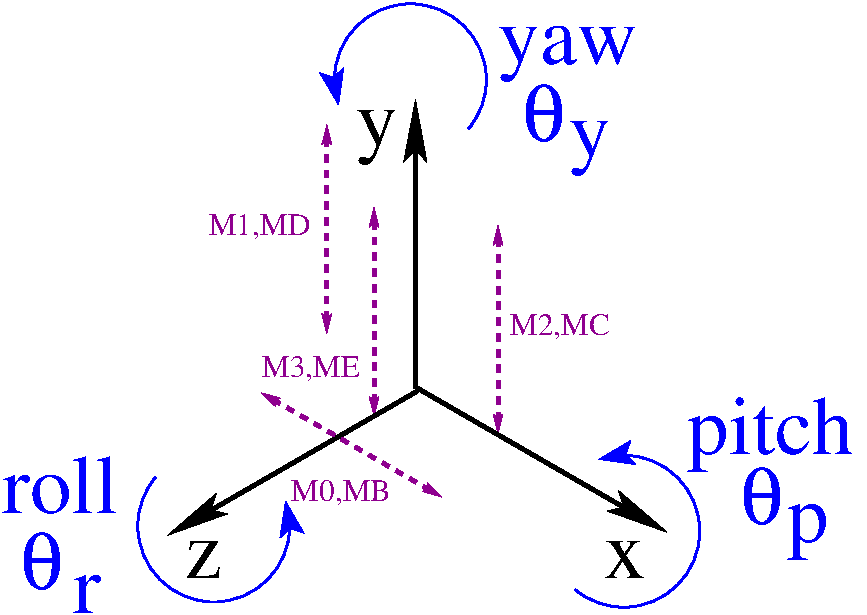
\includegraphics[scale=0.40,angle=0]{fig25.pdf}\caption{Set of movers: M$_{01234}$ in Block IPAB and M$_{BCDE}$ in Block IPC.}\label{f:moverss}
\end{figure}
%\end{column}
%\begin{column}{5.5cm}
\begin{align}
 x &= x_0+f_x(M_{0,B})\label{eq:poscorr}\\
 y &= y_0+f_y(M_{123,CDE})\notag\\
 z &= z_0\notag\\
 \theta_p &= \theta_{p0}+f_p(M_{123,CDE})\notag\\
 \theta_r &= \theta_{r0}\notag\\
 \theta_y &= \theta_{y0}\notag
\end{align}\par

%\end{column}
%\end{columns}\vspace*{0.5cm}
%\begin{columns}
% \begin{column}{5cm}
% \includegraphics[scale=0.25,angle=0]{fig27.pdf}	
% \end{column}
%\begin{column}{5cm}
% \includegraphics[scale=0.25,angle=0]{fig26.pdf}\par
Figure~\ref{f:moverlong} shows the location of the movers along the longitudinal direction. This information is used to calculate the aligment correction limits of the system.\par
\begin{figure}[h]
\centering
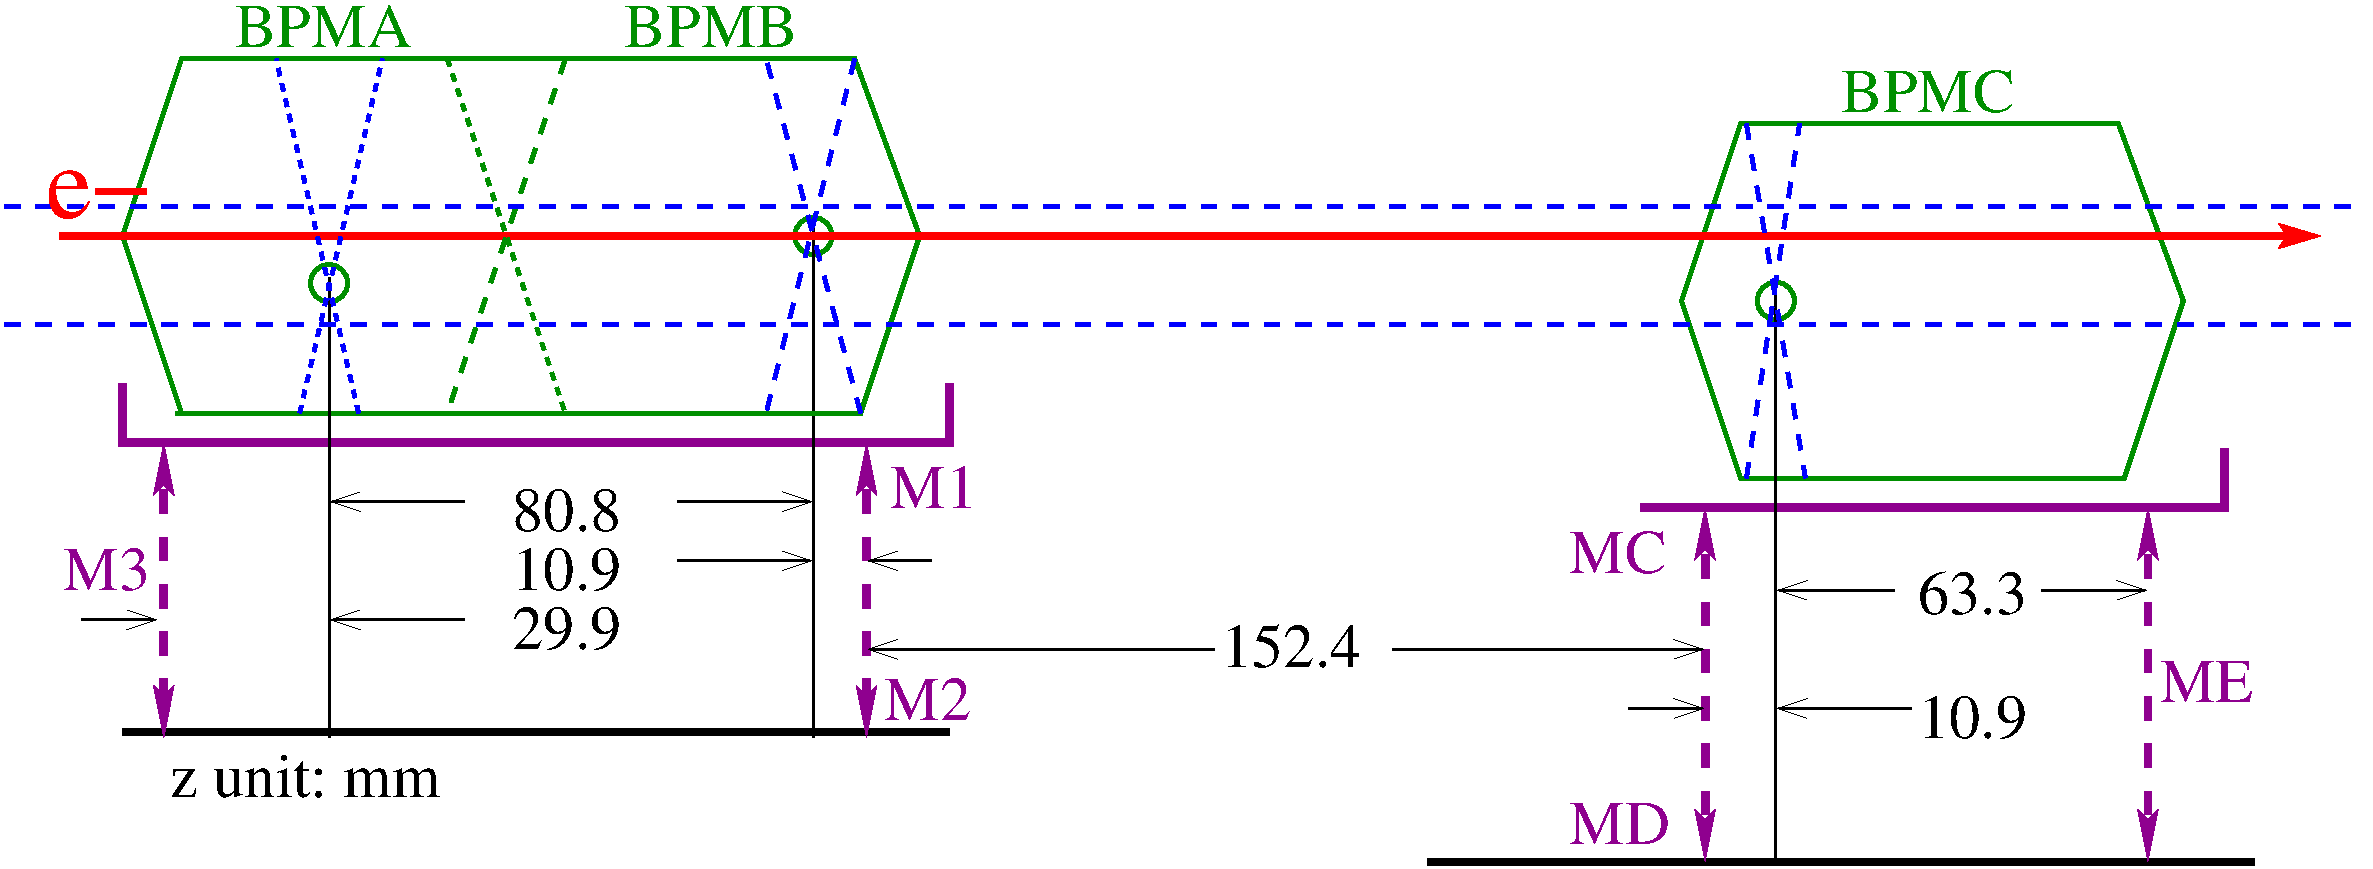
\includegraphics[scale=0.25,angle=0]{fig29.pdf}\caption{Longitudinal position of the movers.}\label{f:moverlong}
\end{figure}
\subsection{Alignment adjustment}\label{s:alignadj}
Normalizing the movers range to -1 to 1 units, as in Eq.~(\ref{eq:Vnorm}), it is possible to calculate the effect of movers  displacement on the cavity position shown in Table~\ref{t:aligncorr}.
\begin{equation}
 M_{0123}=\frac{3-V_{0123}[\text{V}]}{4} \qquad M_{BCDE}=\frac{V_{BCDE}[\text{V}]-5}{5}\label{eq:Vnorm}
\end{equation}
Block IPAB movers are able to correct a maximum of $\pm1$~mrad or $\pm$125~$\mu$m, while Block IPC is able to correct $\pm2$mrad or $\pm$150~$\mu$m. Correction of IPA and IPB position is not independent, therefore, special effort is put into minimize the offset in the block IPAB during installation.\par
By making $y=0$ and $y_0=0$, in Table~\ref{t:aligncorr}, it is also possible to find the ratio of of movers settings that keeps the vertical position and changes the angle per BPM. This gives the possibility to scan sensitivity to pitch angle.\par
\begin{table}[h]
 \centering
 \begin{tabular}{c||c|c|c}\hline
 &\multicolumn{3}{c}{Adjustment}\\\cline{2-4}
 & IPB & IPA & IPC\\\hline\hline
$x$[$\mu$m] & $x_{0B}+{\color{magenta}125M_0}$ & $x_{0A}+{\color{magenta}125M_0}$&${x_{0C}+\color{magenta}150M_{B}}$\\
$y$[$\mu$m]& $y_{0B}+{\color{magenta}11.2M_{1,2}+113.8M_3}$&$y_{0A}+{\color{magenta}94.8M_{1,2}+30.2M_3}$&$y_{0C}+{\color{magenta}128.0M_{CD}+22.0M_E}$\\
$z$[mm]&$z_{0B}$&$z_{0A}$&$z_{0C}$\\
$\theta_{p}$[mrad]& $\theta_{p0B}+{\color{magenta}1.03(M_3-M_{1,2})}$ & $\theta_{p0A}+{\color{magenta}1.03(M_3-M_{1,2})}$ &$\theta_{p0C}+{\color{magenta} 2.02(M_{DC}-M_E)}$\\
$\theta_{r}$[mrad]&$\theta_{r0B}$&$\theta_{r0A}$&$\theta_{r0C}$\\
$\theta_{y}$[mrad]&$\theta_{y0B}$&$\theta_{y0A}$&$\theta_{y0C}$\\\hline
\end{tabular}\caption{Movers setting to adjust position and pitch angle. $M_{0123,BCDE}\in[-1,1]$}\label{t:aligncorr}
% \caption{$M_{0123,BCDE}\in[-1,1],{\color{magenta}\Delta M_{0123,BCDE}}\geq1.25\times 10^{-2}$}\label{t:aligncorr}
\end{table}

\section{Alignment}
\subsection{Vacuum chamber}
The goal is the alignment of the vacuum chamber with respect to external references by less than 200~$\mu$m. Below this range, the piezo-electric movers in each cavity block are used to align the cavity with respect to the beam.\par
The beam positioning system should not interfere with the IPBSM measurements. Therefore, mechanical dimensions and weight should be restricted to those supported by the vertical optical table. This will allow to have a common reference point between the two structures.\par 
\subsection{Effect of alignment on dynamic range}
Dynamic range is reduced by misalignment because of the constant $I'$ and $Q'$ signals from position and angle. This should be minimize aiming to use the maximum dynamic range possible in calibrations and to be near the center of the piezo-movers dynamic range, where linearity is better.\par
However, IPA and IPB are located in a common movers system and therefore BPM position and angle can not be corrected independently. Both BPMs centers can be aligned with the beam by making an angle, but, due the cavity sensitivity to angle of 3.2~$\mu$m/mrad, the $Q'$ will substract the dynamic range available for position scans. This adds to the $Q'$ static signal per BPM and therefore it could become critical.\par
The initial BPM installation \cite{Bambade2013} had alignment issues attributed to loose tolerances between the inner cavity surface and the external reference points \cite{Siwon2014}. During 2014, new cavities were fabricated and installed in the ATF2 line. This set of BPMs has been in use since November 2014.\par
At present there are two methods to check the alignment:
\begin{itemize}
 \item Position scans with $I'=0$. This is fairly simple because it only tries to find the center of the BPM without considering the $Q'$ signal. The issue is that beam angle through the IPBPMs changes and these leads to different alignment results. A typical change of 0.1~mrad in the beam trajectory by a QD0 displacement of 100~$\mu$m could change the aligment results by 25~$\mu$m from IPA to IPC. An incertitude of $\pm10~\mu$m in $I'=0$ has been estimated by analysing different samples in the waveforms. Table~\ref{t:newalign} shows the horizontal and vertical alignment of the new BPMs taken in separated shifts.\par
 \item Position and angle scans to make $I'=0$ and $Q'=0$. First, make $I'=0$ and then use the BPM movers and/or QF7 movers combination to make $Q'=0$. This method is valid for $Q'$ entirely from angle. At the moment it has not been tested with the new BPMs. Table~\ref{t:oldbpms} shows the vertical position results for the previous BPMs. However, the result was corrected after the improvement of the acquisition system. Some initial results in 2013 where resolution limited due to the use of 8 bits oscilloscopes to acquire the waveforms, imposing a resolution limit of the $Q'$ measurement of 1~mrad, which is too large.\par
\end{itemize}
\begin{table}[h]
\centering
 \begin{tabular}{c||c|c|c|l}\hline
  Plane & IPA & IPB & IPC & Comment\\\hline\hline
  X [$\mu$m] & -5 & +18 & -41 & QD0 mover(X)=-70~$\mu$m, 10BX1BY optics\\
  Y [$\mu$m] & -18 & +24 & -102 & QD0 mover(Y)=160~$\mu$m, Low beta optics\\\hline
 \end{tabular}\caption{Alignment measurement using $I'=0$}\label{t:newalign}
\end{table}
\begin{table}[h]
\centering
 \begin{tabular}{c||c|c|c}\hline
 Vertical & IPA &IPB & IPC \\\hline\hline
 Y [$\mu$m] & -7 & +79 & - \\
 $\theta_p$ [mrad] & 0.024 & 1.0& -\\\hline
 \end{tabular}\caption{Alignment measurement using $I'=0$ and $Q'=0$ for previous BPMs.}\label{t:oldbpms}
\end{table}
\subsection{Effect of cavity alignment on calibration}
After the installation the cavities are fixed in the piezo-movers system. Figure \ref{f-BPMcal} shows an static angle $\beta$ between the movers direction and the BPM axis, while the beam makes an angle $\alpha$ with respect to the movers.\par
When doing a position scan to get the BPM calibration the BPM is displaced by $L_m$, however, the displacement seen by the BPM is $L_{BPM}$. Equation (\ref{eq:BPMcal}) shows the effect of the angles in the measured distance and Fig. \ref{f-imagealfabeta} shows the combinations of $\alpha$ and $\beta$ affecting the calibration by less than $10^{-3}$ and $10^{-4}$.\par
Considering $\alpha$, the beam divergence is 0.35~mrad in the nominal optics which is very small and do not affect calibration. The angle change by QF7 has been simulated to have an excursion of 3~mrad at IPB per 1~mm of vertical displacement of QF7, this also remains in below the $10^{-4}$ effect.\par
\begin{figure}[htb]
\centering\hspace*{0.6cm}
\begin{subfigure}{0.4\textwidth}
  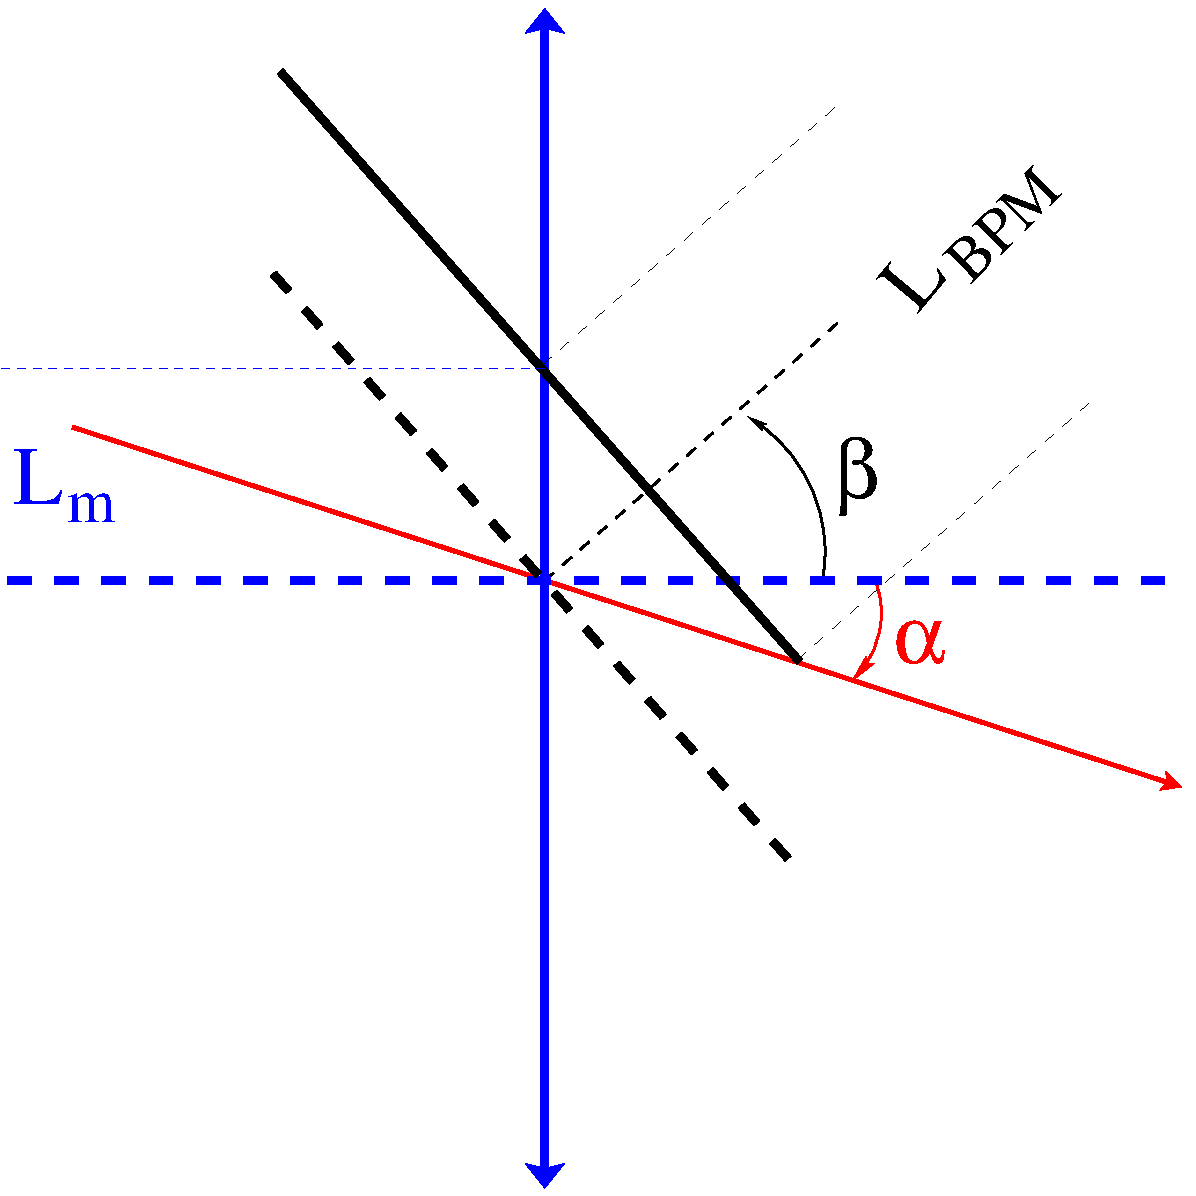
\includegraphics[angle=0,scale=0.26]{BPMcal.pdf}\caption{Displacement from the center. Movers displace by $L_m$. Cavity sees $L_{BPM}$}\label{f-BPMcal}
 \end{subfigure}\hspace*{0.5cm}
 \begin{subfigure}{0.4\textwidth}
  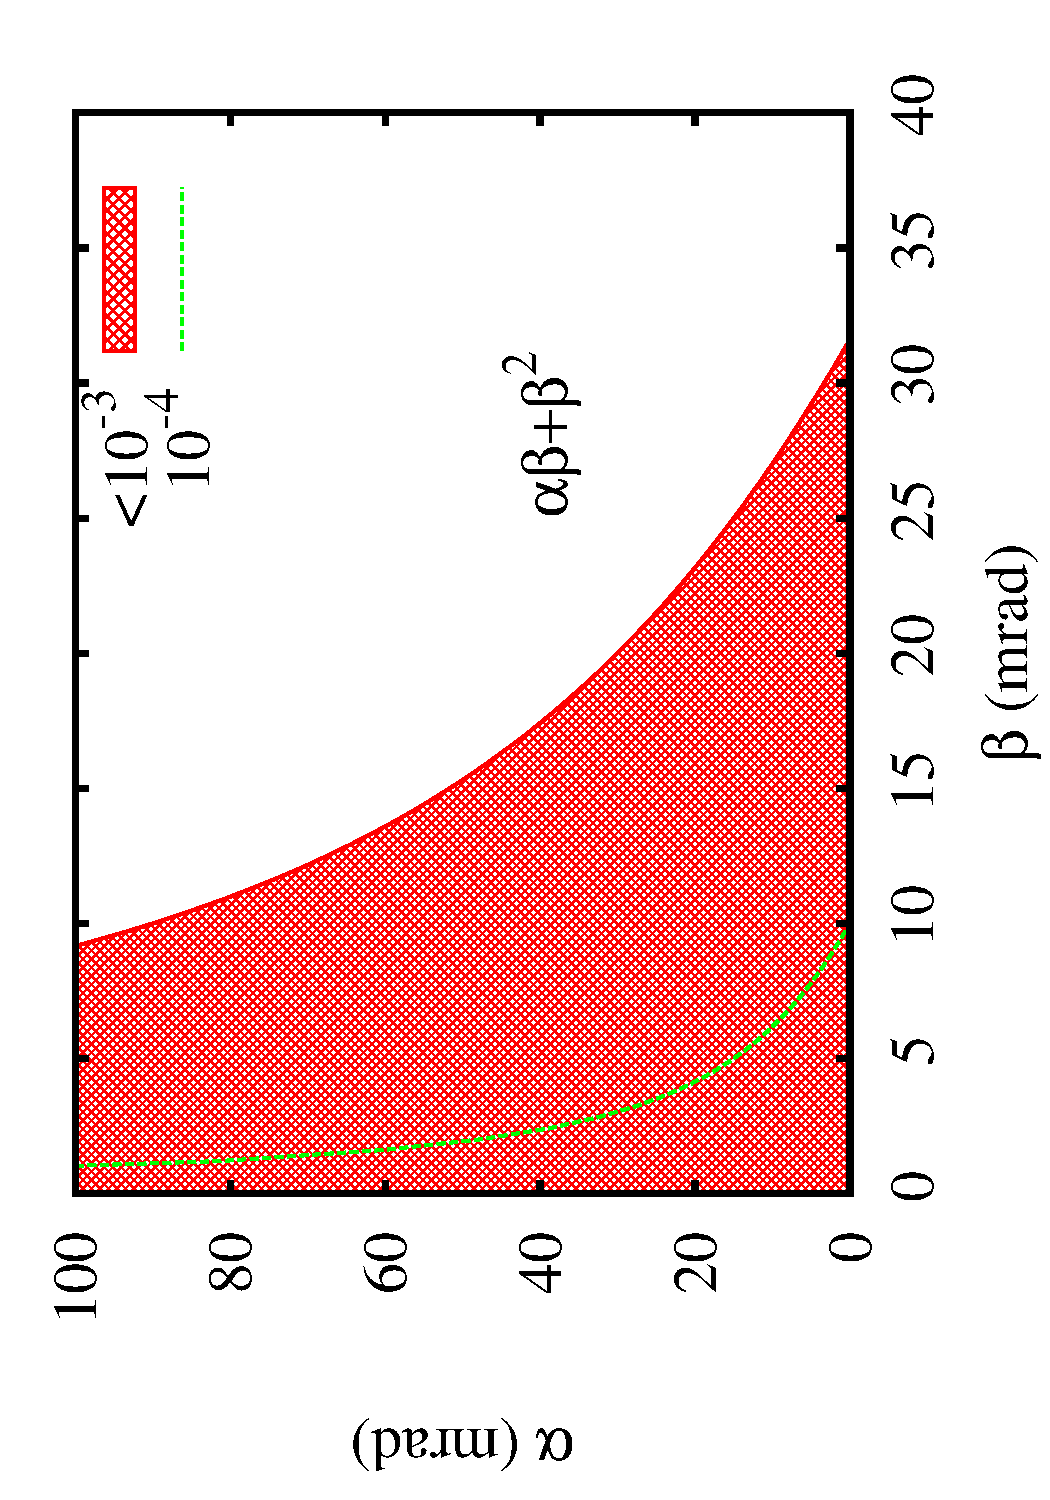
\includegraphics[angle=-90,scale=0.3]{imagealfabeta.pdf}\caption{$\alpha$ and $\beta$ should be inside the dashed area to keep the calibration value within $10^{-3}$ precision.}\label{f-imagealfabeta}
 \end{subfigure}
\end{figure}
\begin{align}
 L_{BPM}=&L_m\left(\cos\beta+\sin\beta\tan(\alpha+\beta)\right)\notag\\
 \approx&L_m(1+\alpha\beta+\beta^2)\label{eq:BPMcal}
\end{align}
If the movers are used to induce an additional angle $\gamma$ to the BPMs as in Fig. \ref{f-BPManglesrot}, then the net effect is and addition of $\beta+\gamma$ shown in Eq. (\ref{eq-BPMcalrot}).\par
\begin{equation}
 L_{BPM}\approx L_m[1+\alpha(\beta+\gamma)+(\beta+\gamma)^2]\label{eq-BPMcalrot}
\end{equation}
The total correction possible for the BPMs is $|\gamma|\leq1$~mrad. It is also a very small angle. The more restrictive angle is $|\beta|<$5~mrad.\par
\begin{figure}[htb]
 \centering
  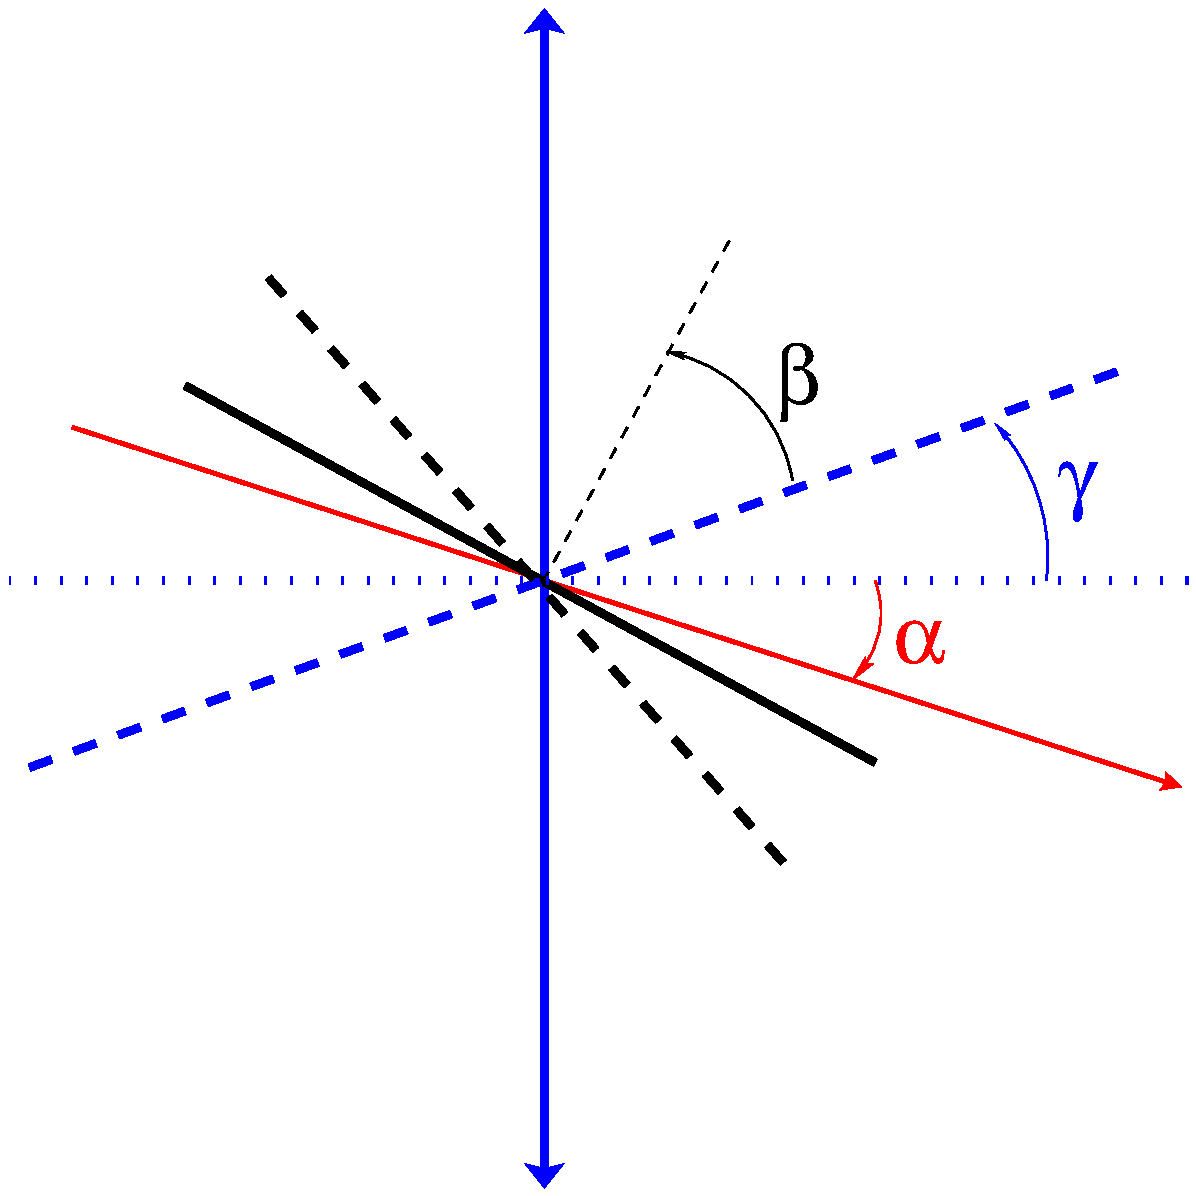
\includegraphics[angle=0,scale=0.3]{BPManglesrot.pdf}\caption{$\gamma$ angle rotation over the BPM. The only effect on distance measured is to add $\gamma$ to $\beta$.}\label{f-BPManglesrot}
\end{figure}
\subsection{Mechanical BPM alignment}\label{s:mechanical}
The estimation of mechanical positions resolution is shown in Table \ref{mechprec}.\par
\begin{table}[htb]
\begin{center}
 \begin{tabular}{|c|c|}\hline
  Axis (Symbol) & Mechanical Precision ($\mu$m)\\\hline
  Vertical ($\Delta y$)& 1\\
  Horizontal ($\Delta x$) & 5\\
  Longitudinal ($\Delta z$) & 5 \\\hline
 \end{tabular}\caption{Position mechanical precision}\label{mechprec}
 \end{center}
\end{table}\par
% Assuming that angles can be estimated from two coplanar points in the BPM, then, minimum resolvable angle might be within the values shown in Table \ref{angleprec}.\par
% \begin{table}[htb]
% \centering
%   \begin{tabular}{|c|c|c|}\hline
%   Angle (Symbol) & Estimated min. resolvable value (mrad) & Distance between points (mm)\\\hline
%    Pitch ($\Delta\theta_p$)&0.042&120\\
%    Yaw ($\Delta\theta_y$)&0.042&120\\
%    Roll ($\Delta\theta_r$)&0.033&30\\\hline
%   \end{tabular}\caption{Angle mechanical precision}\label{angleprec}
% \end{table}
\pagebreak
